% Options for packages loaded elsewhere
\PassOptionsToPackage{unicode}{hyperref}
\PassOptionsToPackage{hyphens}{url}
%
\documentclass[
]{book}
\usepackage{amsmath,amssymb}
\usepackage{lmodern}
\usepackage{iftex}
\ifPDFTeX
  \usepackage[T1]{fontenc}
  \usepackage[utf8]{inputenc}
  \usepackage{textcomp} % provide euro and other symbols
\else % if luatex or xetex
  \usepackage{unicode-math}
  \defaultfontfeatures{Scale=MatchLowercase}
  \defaultfontfeatures[\rmfamily]{Ligatures=TeX,Scale=1}
\fi
% Use upquote if available, for straight quotes in verbatim environments
\IfFileExists{upquote.sty}{\usepackage{upquote}}{}
\IfFileExists{microtype.sty}{% use microtype if available
  \usepackage[]{microtype}
  \UseMicrotypeSet[protrusion]{basicmath} % disable protrusion for tt fonts
}{}
\makeatletter
\@ifundefined{KOMAClassName}{% if non-KOMA class
  \IfFileExists{parskip.sty}{%
    \usepackage{parskip}
  }{% else
    \setlength{\parindent}{0pt}
    \setlength{\parskip}{6pt plus 2pt minus 1pt}}
}{% if KOMA class
  \KOMAoptions{parskip=half}}
\makeatother
\usepackage{xcolor}
\usepackage{color}
\usepackage{fancyvrb}
\newcommand{\VerbBar}{|}
\newcommand{\VERB}{\Verb[commandchars=\\\{\}]}
\DefineVerbatimEnvironment{Highlighting}{Verbatim}{commandchars=\\\{\}}
% Add ',fontsize=\small' for more characters per line
\usepackage{framed}
\definecolor{shadecolor}{RGB}{248,248,248}
\newenvironment{Shaded}{\begin{snugshade}}{\end{snugshade}}
\newcommand{\AlertTok}[1]{\textcolor[rgb]{0.94,0.16,0.16}{#1}}
\newcommand{\AnnotationTok}[1]{\textcolor[rgb]{0.56,0.35,0.01}{\textbf{\textit{#1}}}}
\newcommand{\AttributeTok}[1]{\textcolor[rgb]{0.77,0.63,0.00}{#1}}
\newcommand{\BaseNTok}[1]{\textcolor[rgb]{0.00,0.00,0.81}{#1}}
\newcommand{\BuiltInTok}[1]{#1}
\newcommand{\CharTok}[1]{\textcolor[rgb]{0.31,0.60,0.02}{#1}}
\newcommand{\CommentTok}[1]{\textcolor[rgb]{0.56,0.35,0.01}{\textit{#1}}}
\newcommand{\CommentVarTok}[1]{\textcolor[rgb]{0.56,0.35,0.01}{\textbf{\textit{#1}}}}
\newcommand{\ConstantTok}[1]{\textcolor[rgb]{0.00,0.00,0.00}{#1}}
\newcommand{\ControlFlowTok}[1]{\textcolor[rgb]{0.13,0.29,0.53}{\textbf{#1}}}
\newcommand{\DataTypeTok}[1]{\textcolor[rgb]{0.13,0.29,0.53}{#1}}
\newcommand{\DecValTok}[1]{\textcolor[rgb]{0.00,0.00,0.81}{#1}}
\newcommand{\DocumentationTok}[1]{\textcolor[rgb]{0.56,0.35,0.01}{\textbf{\textit{#1}}}}
\newcommand{\ErrorTok}[1]{\textcolor[rgb]{0.64,0.00,0.00}{\textbf{#1}}}
\newcommand{\ExtensionTok}[1]{#1}
\newcommand{\FloatTok}[1]{\textcolor[rgb]{0.00,0.00,0.81}{#1}}
\newcommand{\FunctionTok}[1]{\textcolor[rgb]{0.00,0.00,0.00}{#1}}
\newcommand{\ImportTok}[1]{#1}
\newcommand{\InformationTok}[1]{\textcolor[rgb]{0.56,0.35,0.01}{\textbf{\textit{#1}}}}
\newcommand{\KeywordTok}[1]{\textcolor[rgb]{0.13,0.29,0.53}{\textbf{#1}}}
\newcommand{\NormalTok}[1]{#1}
\newcommand{\OperatorTok}[1]{\textcolor[rgb]{0.81,0.36,0.00}{\textbf{#1}}}
\newcommand{\OtherTok}[1]{\textcolor[rgb]{0.56,0.35,0.01}{#1}}
\newcommand{\PreprocessorTok}[1]{\textcolor[rgb]{0.56,0.35,0.01}{\textit{#1}}}
\newcommand{\RegionMarkerTok}[1]{#1}
\newcommand{\SpecialCharTok}[1]{\textcolor[rgb]{0.00,0.00,0.00}{#1}}
\newcommand{\SpecialStringTok}[1]{\textcolor[rgb]{0.31,0.60,0.02}{#1}}
\newcommand{\StringTok}[1]{\textcolor[rgb]{0.31,0.60,0.02}{#1}}
\newcommand{\VariableTok}[1]{\textcolor[rgb]{0.00,0.00,0.00}{#1}}
\newcommand{\VerbatimStringTok}[1]{\textcolor[rgb]{0.31,0.60,0.02}{#1}}
\newcommand{\WarningTok}[1]{\textcolor[rgb]{0.56,0.35,0.01}{\textbf{\textit{#1}}}}
\usepackage{longtable,booktabs,array}
\usepackage{calc} % for calculating minipage widths
% Correct order of tables after \paragraph or \subparagraph
\usepackage{etoolbox}
\makeatletter
\patchcmd\longtable{\par}{\if@noskipsec\mbox{}\fi\par}{}{}
\makeatother
% Allow footnotes in longtable head/foot
\IfFileExists{footnotehyper.sty}{\usepackage{footnotehyper}}{\usepackage{footnote}}
\makesavenoteenv{longtable}
\usepackage{graphicx}
\makeatletter
\def\maxwidth{\ifdim\Gin@nat@width>\linewidth\linewidth\else\Gin@nat@width\fi}
\def\maxheight{\ifdim\Gin@nat@height>\textheight\textheight\else\Gin@nat@height\fi}
\makeatother
% Scale images if necessary, so that they will not overflow the page
% margins by default, and it is still possible to overwrite the defaults
% using explicit options in \includegraphics[width, height, ...]{}
\setkeys{Gin}{width=\maxwidth,height=\maxheight,keepaspectratio}
% Set default figure placement to htbp
\makeatletter
\def\fps@figure{htbp}
\makeatother
\setlength{\emergencystretch}{3em} % prevent overfull lines
\providecommand{\tightlist}{%
  \setlength{\itemsep}{0pt}\setlength{\parskip}{0pt}}
\setcounter{secnumdepth}{5}
\usepackage{booktabs}
\usepackage{booktabs}
\usepackage{longtable}
\usepackage{array}
\usepackage{multirow}
\usepackage{wrapfig}
\usepackage{float}
\usepackage{colortbl}
\usepackage{pdflscape}
\usepackage{tabu}
\usepackage{threeparttable}
\usepackage{threeparttablex}
\usepackage[normalem]{ulem}
\usepackage{makecell}
\usepackage{xcolor}
\ifLuaTeX
  \usepackage{selnolig}  % disable illegal ligatures
\fi
\usepackage[]{natbib}
\bibliographystyle{plainnat}
\IfFileExists{bookmark.sty}{\usepackage{bookmark}}{\usepackage{hyperref}}
\IfFileExists{xurl.sty}{\usepackage{xurl}}{} % add URL line breaks if available
\urlstyle{same} % disable monospaced font for URLs
\hypersetup{
  pdftitle={A Reference Manual for the Biostatistics GRA},
  pdfauthor={T. K. Peter},
  hidelinks,
  pdfcreator={LaTeX via pandoc}}

\title{A Reference Manual for the Biostatistics GRA}
\usepackage{etoolbox}
\makeatletter
\providecommand{\subtitle}[1]{% add subtitle to \maketitle
  \apptocmd{\@title}{\par {\large #1 \par}}{}{}
}
\makeatother
\subtitle{Towards readable, rigorous, and reproducible results}
\author{T. K. Peter}
\date{2023-06-19}

\begin{document}
\maketitle

{
\setcounter{tocdepth}{1}
\tableofcontents
}
\hypertarget{motivation}{%
\chapter{Motivation}\label{motivation}}

The meta-question behind this short book is `where to begin?'. I started graduate school in August of 2019, coming straight from an undergrad program in math to a doctoral program in biostatistics. In the same week that I started classes, I started my work as a graduate research assistant in the \href{https://dentistry.uiowa.edu/research/biostatistics-and-computational-biology}{Division of Biostatistics and Computational Biology} at the University of Iowa College of Dentistry. It was a steep learning curve. Now heading into my 5th year as a Ph.D.~student, I began compiling some notes/tips to share with the other graduate research assistants (GRAs) who joined our team after me. Those notes have become this reference manual.

The `first principles' chapter is me diving into the philosophy of why I think this kind of training manual is important. Here, I'll give you the TL;DR: Although a significant component of graduate level study is learning how to learn, brand new GRAs also need to know what to Google. GRAs need to struggle with hard concepts and new ideas -- the learning is truly in the struggle. At the same time, they need to know where to start. This creates a tension: new GRAs need to engage in independent study work, but they also need resources that outline guiding principles. If GRAs don't know what they're searching for, they won't know if they've found it. Moreover, if novice GRAs \emph{think} they know what they are searching for without any guidance, they could easily come across bad advice (by `bad', I mean that which leads to suboptimal outcomes with respect to rigor and reproducibility).

With this tension in mind, the goal of this reference manual is to 1) outline some of the main ideas that you will need to be successful, and 2) to provide you with some vocabulary to help you as you learn independently. Many of the chapters here outline some general concepts and then provide links to further reading.

\hypertarget{what-this-book-assumes}{%
\section{What this book assumes}\label{what-this-book-assumes}}

This is a reference manual, not a formal textbook. As such, my philosophy in writing this is to summarize the most helpful things I have learned in a way that is conducive to quick review. The chapters that are titled after broad areas of research (e.g., `survival analysis') contain more links than new content. I assume throughout this writing that the readers are either familiar with foundational statistical concepts or are currently enrolled in courses that are teaching those concepts.

\hypertarget{acronyms}{%
\section{Acronymns}\label{acronyms}}

Throughout this work, I use the following acronyms:

\begin{itemize}
\tightlist
\item
  \textbf{GRA}: Graduate research assistant
\item
  \textbf{PI}: Primary investigator
\item
  \textbf{CC}: Carbon copy (as in an email)
\item
  \textbf{UI}: University of Iowa
\item
  \textbf{HPC}: High performance computing
\item
  \textbf{SAS}: \href{https://en.wikipedia.org/wiki/SAS_(software)}{Statistical Analysis System} software
\item
  \textbf{GWAS}: Genome-wide association study
\item
  \textbf{QC}: quality control
\end{itemize}

\hypertarget{working-with-the-garage-door-open}{%
\section{Working with the garage door open}\label{working-with-the-garage-door-open}}

This manual is a work in progress. I am writing this as I work my way through my own program, making notes as I go. This is in the spirit of \href{https://notes.andymatuschak.org/About_these_notes?stackedNotes=z21cgR9K3UcQ5a7yPsj2RUim3oM2TzdBByZu}{working with the garage door open}, an approach to learning that really resonates with me.

Keep in mind that as I'm writing this, I am also a student myself. I want to make improvements to this manual as I keep learning. If you think of a reference that you'd like to see included, open a GitHub issue or make a pull request to let me know. I would welcome any feedback, and would appreciate any thoughtful critiques.

\hypertarget{acknowledgements}{%
\section{Acknowledgements}\label{acknowledgements}}

So much of this work comes directly from what I have learned from my dissertation advisor \href{https://myweb.uiowa.edu/pbreheny/}{Patrick Breheny} and my GRA supervisor \href{https://scholar.google.com/citations?hl=en\&user=flqLOJIAAAAJ}{X. Jin Xie}. Both of these men have had a tremendous influence on my thinking.

I also want to thank the other UI biostats professors who have taught my core courses; our department is stacked with faculty who are dedicated teachers as well as brilliant researchers.

\hypertarget{dedication}{%
\section{Dedication}\label{dedication}}

This work is dedicated in loving memory of my father, \href{https://www.hendersonvillefh.com/obituary/William-Peter}{Bill Peter} (1955-2022).

\hypertarget{first-principles---invisible-and-integral-work}{%
\chapter{First Principles - invisible and integral work}\label{first-principles---invisible-and-integral-work}}

There are professions in which excellence brings invisibility. In such professions, the reward of a job well done is the unnoticed reception of the work into the foundation of the organization which the worker supports. Successes are silent, while failures are deafening.

An illustrative example of this phenomena is observed in custodial work. Custodial staff members know that when their job is done well, no one will notice. However, when their job is undone or done poorly, \emph{everyone} will notice.\footnote{I borrow this example from a phrase often used by my late grandmother (my father's mother), Jean, who was a housekeeper in a hospital.} The work in such professions is both integral and invisible. I argue that the field biostatistics epitomizes this phenomena. We who work as biostatisticians are called upon to work in humility, willing to invest much in the invisible and integral art of communicating the truth in this data-saturated historic moment.

This work is a reference manual, which means most of its contents are not new. Rather, the novelty in what I am providing here is in its form and organization. As a 4th year PhD student, I set out to gather resources together to help the newer GRAs on my team, with the goal of helping them by sharing the links, lectures, and tips that have helped me the most. What I am publishing here is the result of that work. Although this reference manual is intended to serve graduate students and early career professionals in biostatistics, I think many of those working in the fields of statistics, data science, and bioinformatics may resonate with the calling to work in invisible and integral spaces and find this manual relevant to their work.

The objective of this manual is twofold: to provide starting points from which to address common questions of practice, and to summarize the references and tools which I have found most helpful in my journey through gradate school and my early years as a biostatistician. Overarching these two goals is a desire to make a contribution toward training biostatisticians whose work is readable, rigorous, and reproducible.

If even one other person is encouraged and sharpened by this work, my goal will be accomplished.

Yours faithfully,
TKP

2023

\hypertarget{getting-organized-the-first-3-days-of-a-new-ra-job}{%
\chapter{Getting organized: The first 3 days of a new RA job}\label{getting-organized-the-first-3-days-of-a-new-ra-job}}

The first step in starting out as a research assistant is establishing habits of organization. American author O. S. Marden said it this way: ``A good system shortens the road to the goal.'' You will be more productive and produce higher quality work -- work that is reproducible and rigorous -- if you begin by establishing an organizational system.

I will outline here both general principles and some specific strategies that have proven helpful for my work. These points are organized according to the three major components to your work system that should be established within your first few days on the job:

\begin{enumerate}
\def\labelenumi{\arabic{enumi}.}
\item
  File structure
\item
  Emails
\item
  Notes and README files
\end{enumerate}

\hypertarget{file-structure}{%
\section{File structure}\label{file-structure}}

`File structure' refers to the system for categorizing your code, notes, reports, and figures for each project. Here are some general principles:

\begin{enumerate}
\def\labelenumi{\arabic{enumi}.}
\tightlist
\item
  One master folder per project
\end{enumerate}

\begin{itemize}
\tightlist
\item
  the `master folder' structure translates well to starting GitHub repositories {[}CROSS REF{]}.
\end{itemize}

\begin{enumerate}
\def\labelenumi{\arabic{enumi}.}
\setcounter{enumi}{1}
\tightlist
\item
  Subfolders for each file type
\end{enumerate}

\begin{itemize}
\tightlist
\item
  keeping subfolders by file type will help you find what you are looking for. Also, doing it this way will let you script your work from the command line with ease -- for example, you can apply a function or use an executable file to work with all the items in a given folder.
\end{itemize}

\begin{enumerate}
\def\labelenumi{\arabic{enumi}.}
\setcounter{enumi}{2}
\tightlist
\item
  Names that are readable for both humans and machines
\end{enumerate}

\begin{itemize}
\tightlist
\item
  use names that can be easily ordered by a computer; again, this helps with writing scripts.
\item
  avoid using white spaces, as this is a hassle for machines to read. Choose to work with either `CamelCase' or `snake\_case', and be consistent.
\item
  use specific keywords in file names: `tkp\_edited\_version' is better than `final\_version'
\item
  it's worth saying again: choose a convention and be consistent
\item
  one more time for the folks in the back: choose a convention and \textbf{be consistent}.
\item
  for a brief (and entertaining) tutorial on naming things, checkout \href{https://www.youtube.com/watch?v=ES1LTlnpLMk}{Jenny Bryan's YouTube video}.
\end{itemize}

\begin{enumerate}
\def\labelenumi{\arabic{enumi}.}
\setcounter{enumi}{3}
\tightlist
\item
  Example
\end{enumerate}

Here is a step-by-step example of how I use a file structure to organize myself at the start of a new project (if you'd prefer, \protect\hyperlink{folder-video}{skip to the video}). Suppose I am contacted by Collaborator A for support on a study of a new endodontic treatment\ldots{}

\begin{enumerate}
\def\labelenumi{\arabic{enumi}.}
\item
  I begin by creating a new folder with a name that fits my established convention. For my new project, I would create a folder \texttt{TKP23-A-Endo}. My folders are stored in a shared drive to which other biostatistician have access, so I begin my folder names with my initials (TKP). the `23' tells me that the project started in 2023. The `A' and `Endo' keywords tell me who is the PI/what project it is (this is helpful since it is not uncommon for me to have multiple projects from the same lab).
\item
  The first file I add to my new \texttt{TKP23-A-Endo} folder is a \protect\hyperlink{readme}{README file}. This includes notes from the initial meeting/first email from Collaborator A.
\item
  I open \href{https://posit.co/download/rstudio-desktop/}{RStudio} and go to \texttt{File\ \textgreater{}\ New\ Project}. I follow the prompts to create a new project, and the directory (a.k.a the folder) in which this project will live is my new \texttt{TKP23-A-Endo} folder. Using an R project is an example of a broader principle of \href{https://www.tidyverse.org/blog/2017/12/workflow-vs-script/}{project-oriented workflow}.
\item
  I go to my \texttt{TKP23-A-Endo} folder (which now has two things in it: a \texttt{.Rproj} file and a \texttt{README} file), and I make 4 subfolders: \texttt{data}, \texttt{scripts}, \texttt{reference}, and \texttt{reports}. These are the building blocks of my projects.
\end{enumerate}

\begin{itemize}
\item
  I will get data from Collaborator A, and it will go in the data folder. \textbf{Nothing else} will go in the data folder, and I will never change any original files in the data folder. If I need to edit the data in some way (this is esp.~relevant when data come in the form of Excel), I make a copy of the files I want to change and then work with those copies.
\item
  \texttt{scripts} will be the place where I put all of the code I use for data cleaning and analysis.
\item
  \texttt{reference} is where I will put things Collaborator A shares with me that help me understand the research question -- this could be articles in endodontics that provide an explanation of the terminology, or a PowerPoint that explains how the data are collected. I would also keep a copy of the \href{https://www.fda.gov/regulatory-information/search-fda-guidance-documents/institutional-review-boards-frequently-asked-questions}{IRB} documentation in this \texttt{reference} folder.
\item
  \texttt{reports} is where I will keep my final \texttt{.Rmd} file for writing the report which I will share with Collaborator A.
\end{itemize}

From here, I begin writing scripts.

\begin{enumerate}
\def\labelenumi{\arabic{enumi}.}
\setcounter{enumi}{4}
\tightlist
\item
  As the project moves along, I may find that I need other subfolders. For instance, a \texttt{graphics} subfolder would be useful if I am making a ton of plots for a project. If I am writing a manuscript and there's quite a bit of back-and-forth with reviewers, I would use a \texttt{submission} subfolder that contains all my point-to-point responses (CROSS REF) for reviewers.
\end{enumerate}

\hypertarget{folder-video}{%
\subsection{Folder setup video}\label{folder-video}}

\href{https://youtu.be/4UxoLIOmkzc}{Here's a short YouTube video} that gives an overview of my typical project folder setup.

\hypertarget{please-use-relative-file-paths}{%
\subsection{Please use relative file paths}\label{please-use-relative-file-paths}}

Computers work with files by having a `pointer' at a specific folder, called a \emph{directory}. Your computer probably has many directories on it -- for example, `Desktop' and `Downloads' are both directories you have by default in a Mac operating system. When you are doing project-based quantitative work, your scripts (the files with the code in them) will need to `point' to data that is probably in another place. Instead of copying data into multiple folders, or using functions like \texttt{setwd()}, use \emph{relative filepaths}. This can be accomplished using the \texttt{..} symbol to reference a \emph{parent directory}. \href{https://youtu.be/eb11iggmuwM}{Here is a short video} on how I use relative file paths.

\hypertarget{emails}{%
\section{Emails}\label{emails}}

Email management is of paramount importance for collaboration. Emails serve 2 purposes:

\begin{itemize}
\item
  Providing a paper trail to document important exchanges of information
\item
  Facilitating conversations that can happen in an asynchronous way
\end{itemize}

I have found the \href{https://hive.com/blog/inbox-zero/}{Inbox Zero method} for email management to be a helpful place to begin. This method breaks down emails in to 4 categories: delete, delegate, defer, and do. Practically speaking, I have folders named for each person with whom I correspond. When I receive a new email that needs an answer, this goes in a `needs follow up' folder. After following up, I move the conversation to the folder with the appropriate name (with group conversations categorized by the PI).

I \textbf{do not recommend} using emails to exchange versions of important files. Several tools exist to facilitate collaboration in a more efficient way - Microsoft offers `OneDrive', Google offers `GoogleDrive', and of course, there's \href{https://docs.github.com/en/get-started/getting-started-with-git}{GitHub}. In addition, most organizations have a some kind of shared drive/shared repository. As often as possible, use shared resources for file sharing as opposed to emailing different versions.

\hypertarget{organizing-your-inbox}{%
\subsection{Organizing your inbox}\label{organizing-your-inbox}}

Here's a short video on how to organize your inbox:

TODO: add video here!

\hypertarget{project-notes}{%
\section{Project notes and README files}\label{project-notes}}

You have to keep track of what you are learning. In addition, you need to keep a log of what you have done so that other collaborators/future RAs can look back and figure out what you did. Let's call these two tasks \emph{internal} documentation (keeping track of your project-specific work) and \emph{external} documentation (the project-specific notes you want to leave for others). I recommend writing project notes for internal documentation, and README files for external documentation.

\hypertarget{project-notes-1}{%
\subsection{Project notes}\label{project-notes-1}}

Each project is a process that unfolds over time. As you learn over the course of a project, you'll need some kind of time-organized system for keeping track of your thoughts and action items. Using Google Drive, I have created a system of weekly project notes to serve this purpose. The setup looks like this:

\begin{figure}
\centering
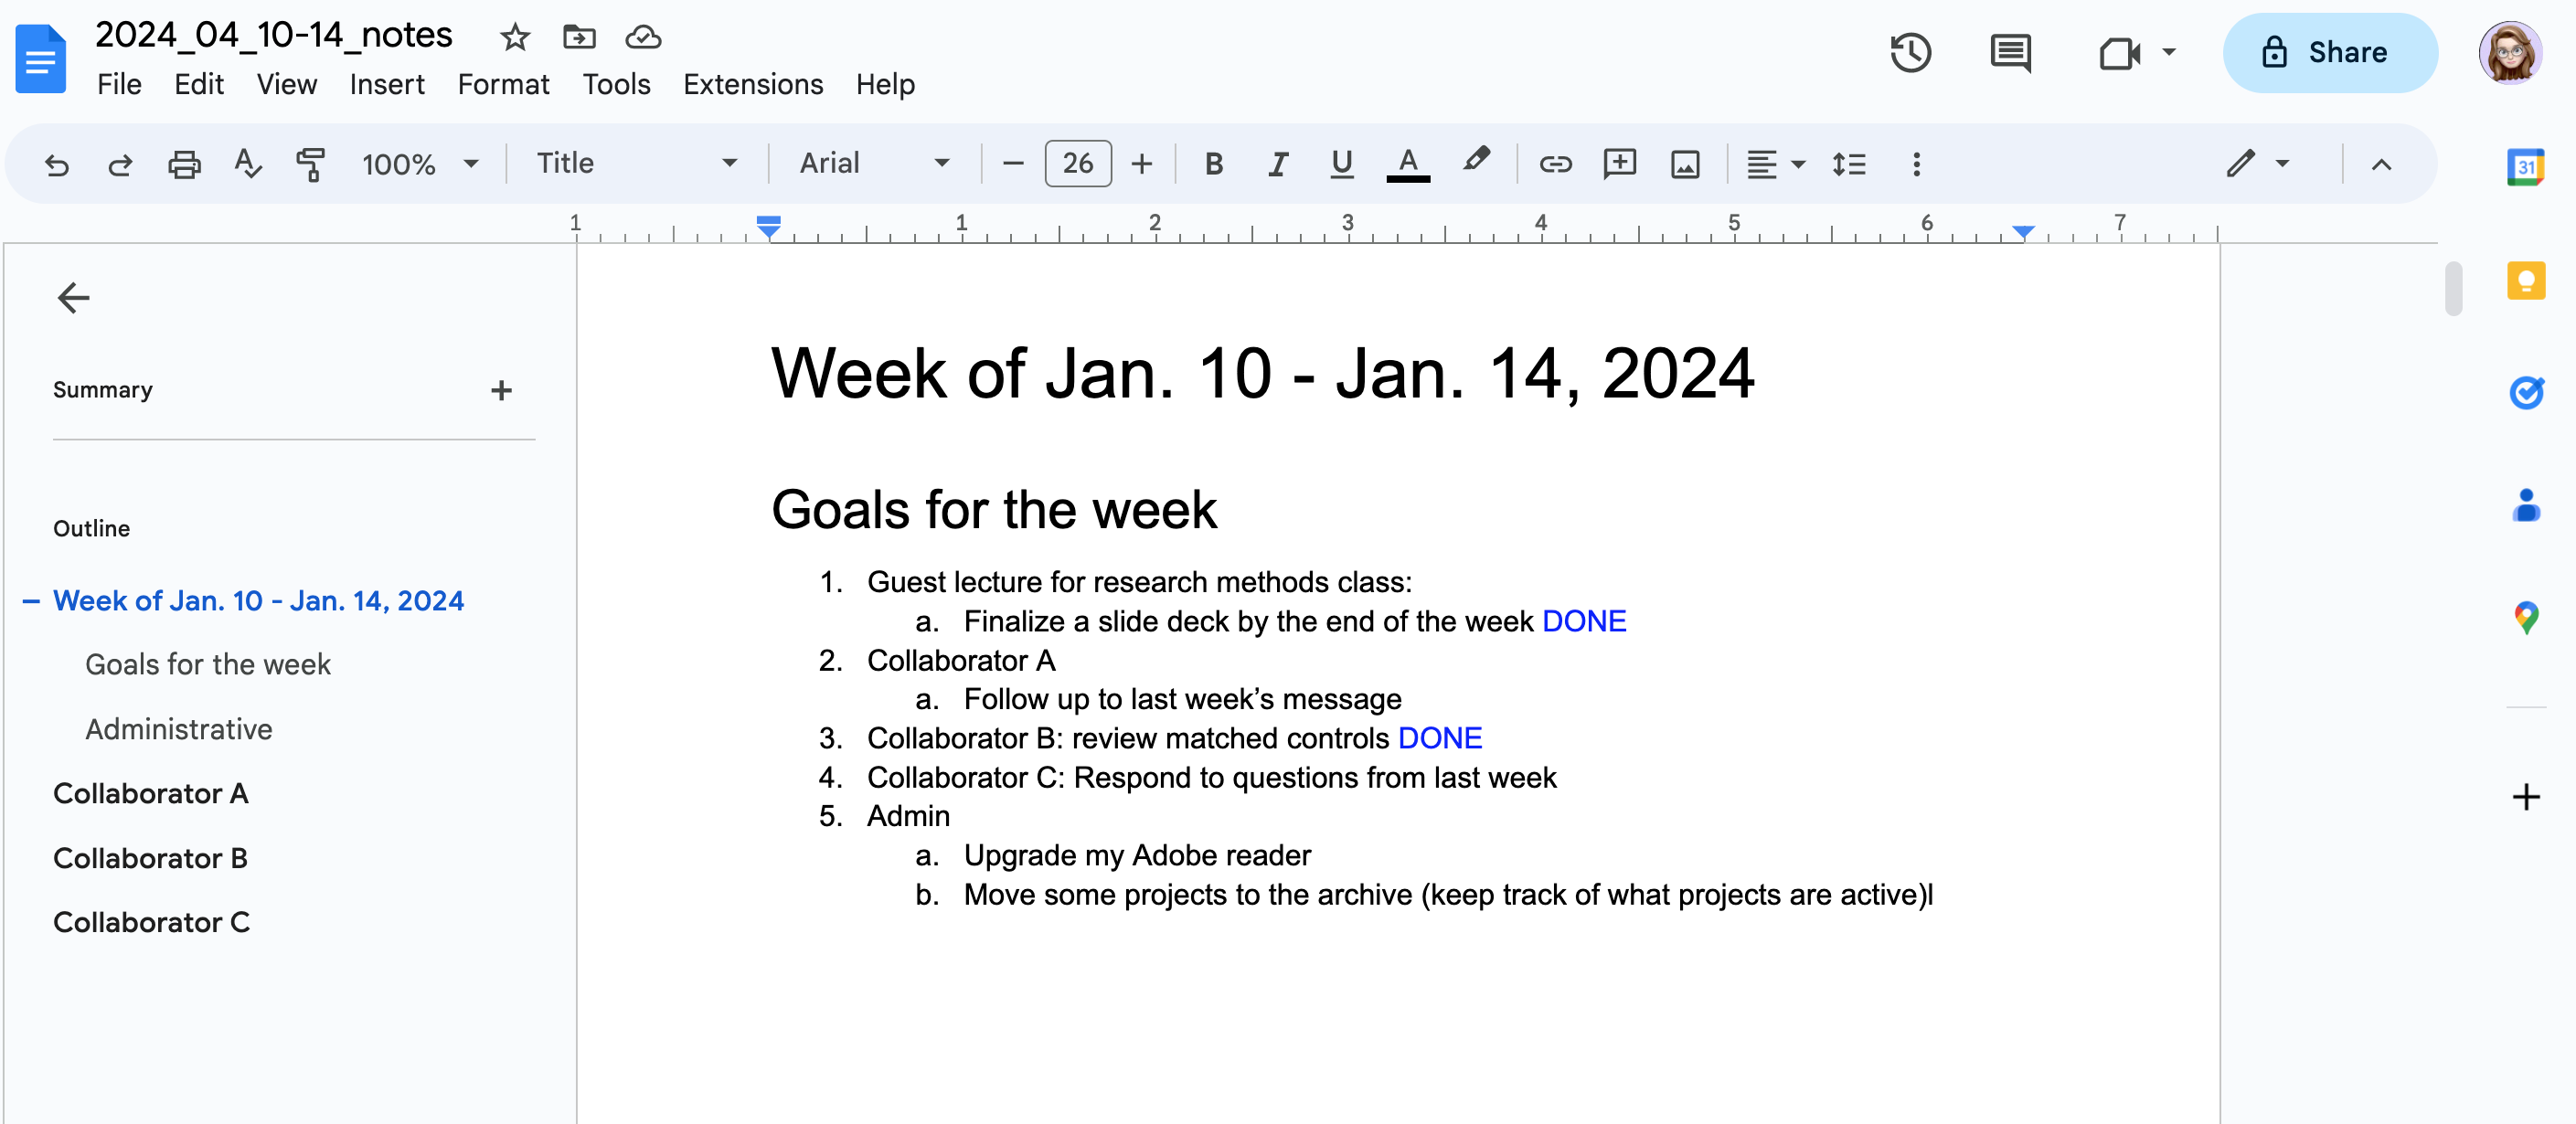
\includegraphics{img/weekly_notes.png}
\caption{Weekly notes template}
\end{figure}

Each week (typically on Monday morning), I create a new Google doc file named \texttt{YYYY\_MM\_DD1-DD2\_notes} (YYYY = year, MM = month, DD1-2 = dates of Monday \& Friday). On the first page, I set goals for the week. I check off things that are completed by marking them as done. Colored fonts help me stay organized, especially in seasons where I have several collaborative projects going on concomitantly. I often use blue text to show things that are done, and red text to show deadlines.

At the left panel, you can see that each subsequent page of my document is given a subheading link with the collaborator's name. To navigate to my notes for each collaborator, I can use these subheading links to quickly find what I am looking for. If I click on Collaborator A, I would see this page:

\begin{figure}
\centering
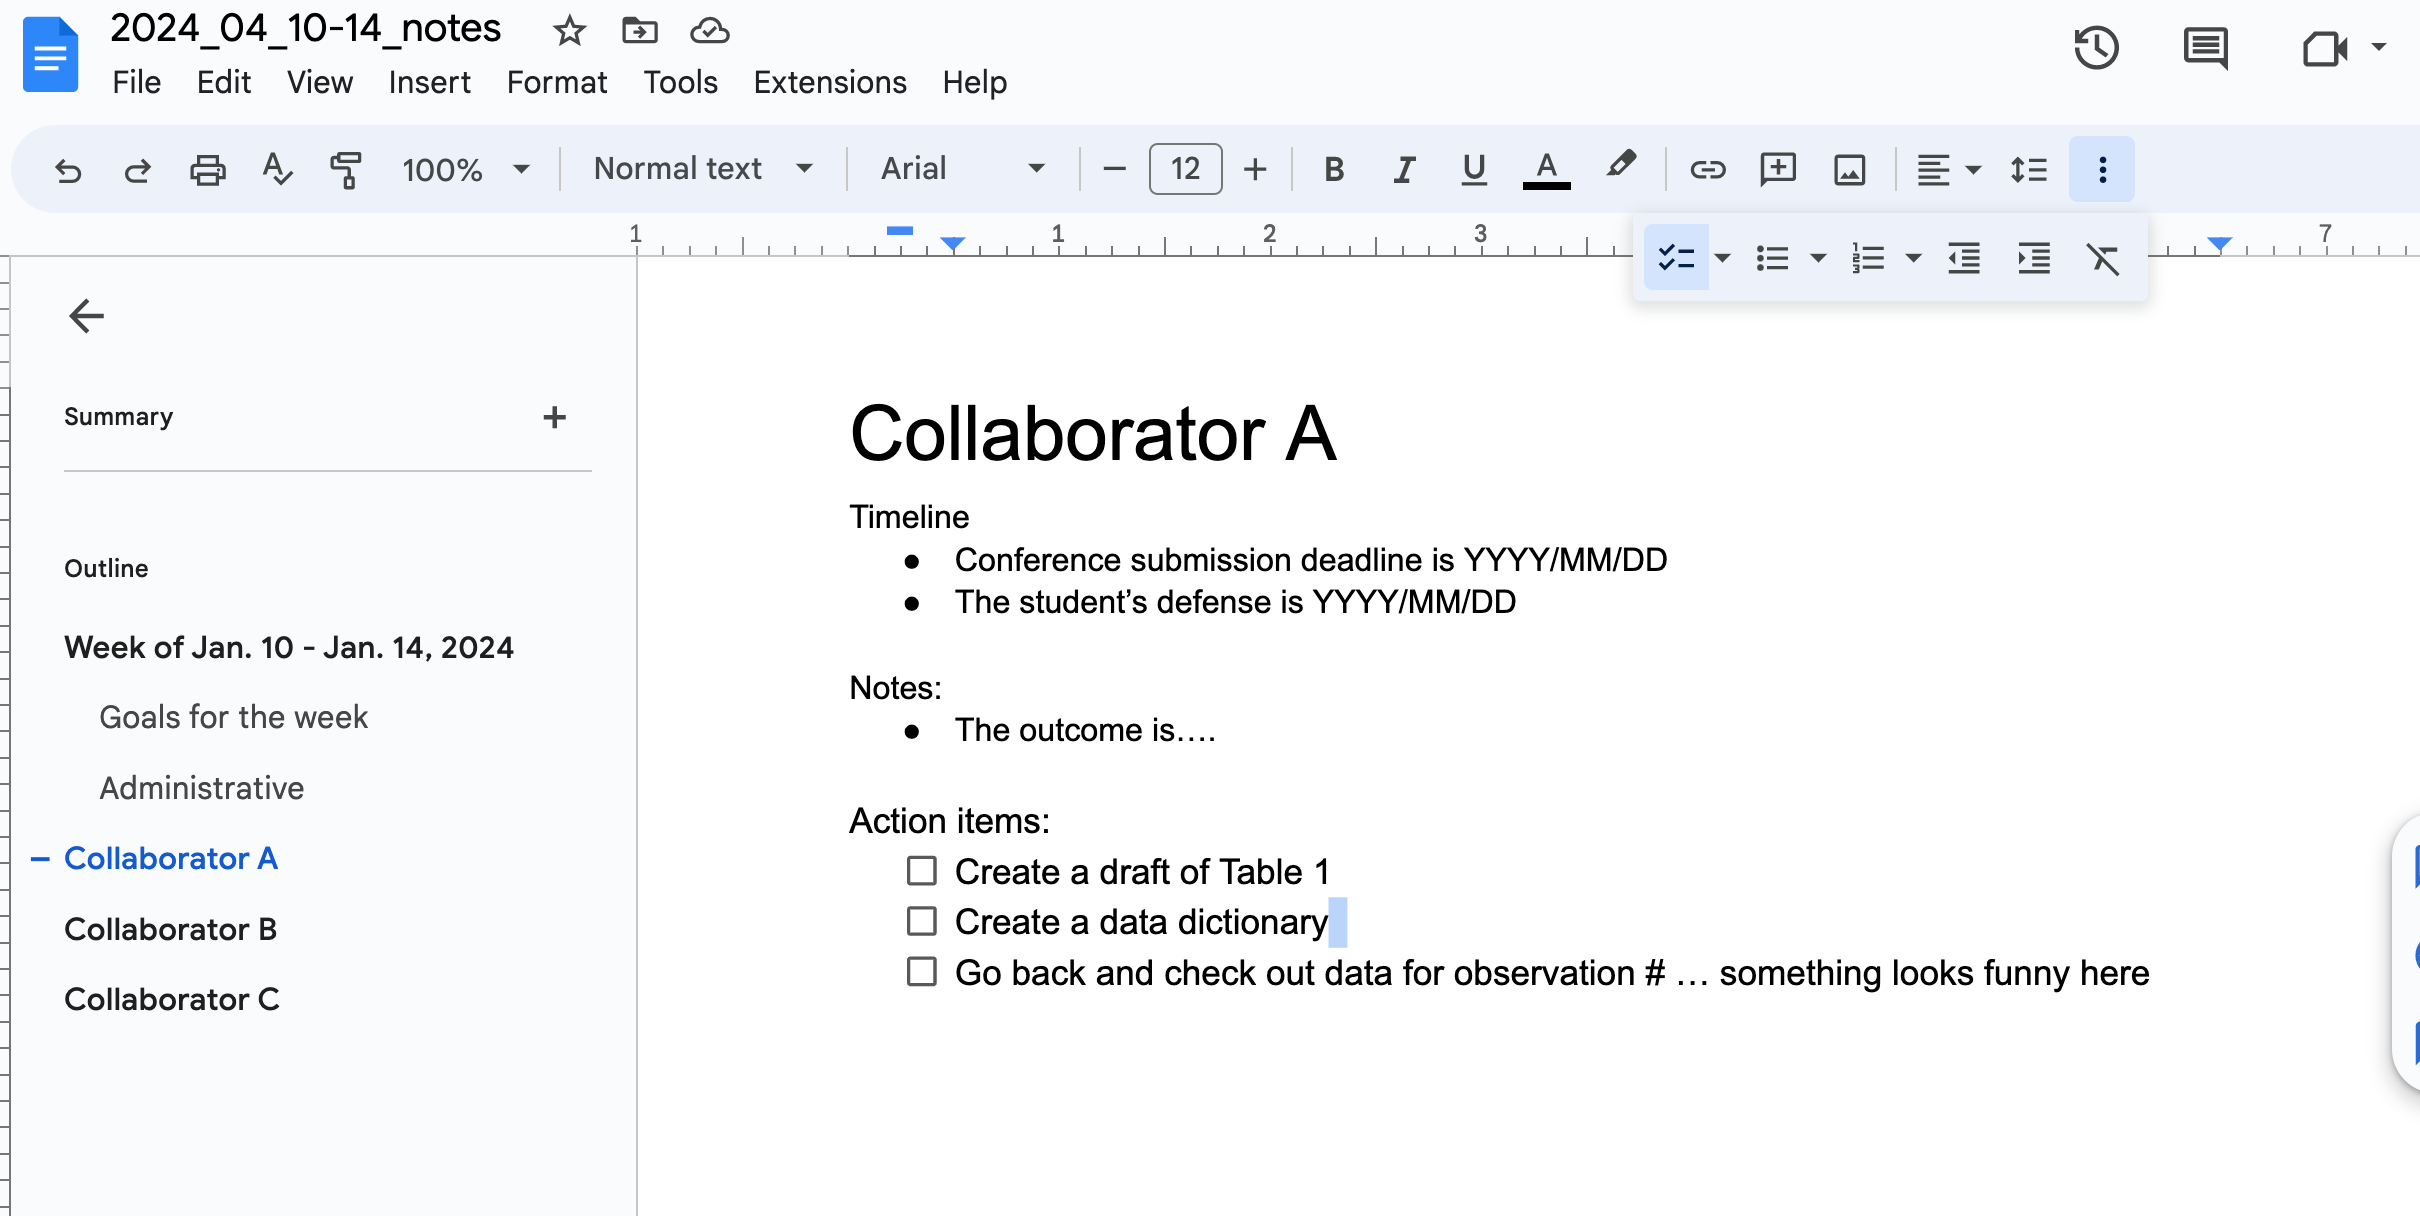
\includegraphics{img/weekly_notes2.png}
\caption{Detail notes for a specific collaborator}
\end{figure}

My notes for each project are typically sorted into times/deadlines, notes, and action items. Whereas my weekly goals are different each week, I probably won't address all the action items for each project in a given week. The notes on this ``Collaborator A'' page may are updated only as often I am working on this project/in contact with the collaborator.

At the start of the next week, I begin my copying the notes from the previous week (the whole file) and then updating the weekly goals. This is an iterative process, where the `current' value becomes the `old' value in the next iteration.

This system of file keeping has allowed me to focus my goals for each week, to measure the progress I am making, and to reference projects that resurface after a long break (which is typical). No one else has access to these notes except me, and I write them in `shorthand' (using acronyms, etc.) knowing that these notes are just for my personal reference.

Notice that these notes are both 1) linear (chronological) and 2) project-specific. These features differentiate project notes from \protect\hyperlink{zettelkasten}{building a personal knowledge base}. Personally, I have found it helpful to keep these two types of notes distinct. My project notes have lots of deadlines, dates, and to-do items -- I don't want these things to get mixed up into my personal knowledge base notes.

\hypertarget{readme}{%
\subsection{README files}\label{readme}}

Each project on which I collaborate has a README file, which has the details that a future analyst would need to jump into a project mid-story. Typically, my README files contain:

\begin{itemize}
\item
  The names of the PI/collaborators
\item
  The objective/scientific aim of the project
\item
  The definitions of any project-specific acronyms
\item
  Any notes on data analysis decisions (i.e., dichotomizing a continuous variable, etc.). Often, these notes are lines from an important email that I copy \& paste into the README. This keeps a coherent record of the decision points in a project timeline.
\end{itemize}

For a deeper dive on writing README files, check out \href{https://www.freecodecamp.org/news/how-to-write-a-good-readme-file/}{this tutorial article}.

\hypertarget{taking-notes}{%
\chapter{Taking Notes}\label{taking-notes}}

One of the most important aspects of studying at the graduate level is taking notes so as to \textbf{build a knowledge base}. Unlike taking notes in other contexts (like undergrad), the goal for a graduate student/GRA is not to keep a linear track of what you've learned over a finite period of time. In undergraduate classes, you take notes per lecture, per week, with the objective being a final at the end. You probably never look back to the notes for any particular class once the semester is over. But graduate school note taking has an altogether different goal. Instead of tracking what you are learning in a linear way for a finite time, you are building up what you are learning into a knowledge base to be referenced for the rest of your life.

So, I highly recommend that you take notes in a way that helps you connect concepts across coursework and RA work. During my 3rd year of grad school, my advisor shared some of his note-taking strategies with me. These strategies transformed the way I learn. Here are some of the ideas that led to that transformation.

\hypertarget{zettelkasten}{%
\section{The Zettlekasten system}\label{zettelkasten}}

One \href{https://en.wikipedia.org/wiki/Note-taking\#Non-linear_note-taking}{non-linear note taking approach} is the \href{https://zettelkasten.de/posts/overview/}{Zettelkasten method}. The \href{https://writingcooperative.com/zettelkasten-how-one-german-scholar-was-so-freakishly-productive-997e4e0ca125}{Writing Cooperative has an article} that describes the Zettlekasten system of taking notes. The Zettelkasten method allows you to connect your notes to one another, so that you end up with a web of ideas. This web is similar to the way Wikipedia is set up, with pages linked to other pages. Other variants of this kind of note taking include \href{https://maggieappleton.com/garden-history}{digital gardening} and \href{https://notes.andymatuschak.org/Evergreen_note-writing_as_fundamental_unit_of_knowledge_work?stackedNotes=z4SDCZQeRo4xFEQ8H4qrSqd68ucpgE6LU155C}{Evergreen notes}.

\hypertarget{how-to-connect-your-notes}{%
\section{How to connect your notes}\label{how-to-connect-your-notes}}

So, this raises the question: where do you start in building up a knowledge base like this? I use the free app called \href{https://obsidian.md/}{Obsidian}. Obsidian allows you to store all your notes in Markdown files on your local machine. There are other apps out there, like \href{https://roamresearch.com/}{Roam}. Just keep in mind that Roam does not have a free version (as of the time of this writing).

Some people who use this kind of note-taking system have made their notes publicly available. I have learned much from studying these peoples' notes:

\begin{itemize}
\item
  \href{https://notes.andymatuschak.org/About_these_notes}{Andy Matuschak}
\item
  \href{https://maggieappleton.com/notes}{Maggie Appleton}
\item
  \href{https://publish.obsidian.md/bryan-jenks/Z/INDEX}{Bryan Jenks}
\end{itemize}

\hypertarget{cultivating-professionalism}{%
\chapter{Cultivating professionalism}\label{cultivating-professionalism}}

\hypertarget{data-management}{%
\section{Data management}\label{data-management}}

Many graduate research assistants have data management responsibilities in addition to data analysis. \href{https://www.oracle.com/database/what-is-data-management/}{Oracle} defines data management as the ``\ldots practice of collecting, keeping, and using data securely, efficiently, and cost-effectively.'' Based on \href{https://people.umass.edu/biostat690c/pdf/1.\%20\%20Principles\%20of\%20Data\%20Management\%202020.pdf}{these notes from the University of Mass.}, here are the general components of data management:

\begin{enumerate}
\def\labelenumi{\arabic{enumi}.}
\item
  Write a data management plan
\item
  Specify a explicit set of operating procedures
\item
  Create a data dictionary
\item
  Determine a data storage location
\item
  Develop an analysis plan
\item
  Archive all of your procedures
\end{enumerate}

I expand on each of these items below:

\hypertarget{write-a-data-management-plan}{%
\subsection{Write a data management plan}\label{write-a-data-management-plan}}

As soon as you receive a new project, you should establish your organization system {[}CROSS REF{]}. After this, your next step should be to spend some time contemplating a data management plan. This plan should describe how you will keep track of all of the data so that you can explain each step of your analysis process.

If collected data comes to you (especially if it comes via an Excel spreadsheet), you should immediately make a copy of this data. \textbf{You should never edit the original data you receive} - do not do any data cleaning or re-formatting. Instead, do all of your work on the copy, so that you can always refer back to the original data.

If you are planning a study with yet-to-be- collected data, spend some time thinking about how the data will get to you.

\begin{itemize}
\item
  Will the data come from electronic records? If so, save the SQL query/other code used to extract the records.
\item
  Will the data come from a chart review (e.g., a doctor will manually collect data from patient records)? If so, I recommend making a template for the doctor (or whoever is doing the chart review) to fill in.
\item
  Think about each person who will interact with the data, and have a flow-chart in your mind that traces exactly how this data will come to you. This will help you when you write the ``Methods'' section of your paper/poster, and will keep you from making mistakes in your analysis downstream.
\end{itemize}

\hypertarget{specify-a-explicit-set-of-operating-procedures}{%
\subsection{Specify a explicit set of operating procedures}\label{specify-a-explicit-set-of-operating-procedures}}

If you are in a situation where multiple people will handle the data (as in the chart review scenario), you should go beyond `having a flow chart in your mind' -- in cases like these, write down who will do what with the data at each step of data collection. Send this written document to everyone on the team, and make sure everyone agrees/is on the same page.

If you are in the chart review scenario, instruct the person doing chart review on how to collect data that is in a consistent form. Remember that the computer will recognize these responses as four different values: ``Yes'', ``yes'', ``y'', ✅.

\hypertarget{create-a-data-dictionary}{%
\subsection{Create a data dictionary}\label{create-a-data-dictionary}}

Create a spreadsheet with all the variables in the study listed in one column, and their definitions listed in the next column. As you write your scripts for analysis, you may even want to add a third column that lists the name you used in the script for that variable. \href{https://data.nal.usda.gov/manually-creating-data-dictionary}{The US Dept. of Agriculture} offers some best practices on organizing a data dictionary.

\hypertarget{determine-a-data-storage-location}{%
\subsection{Determine a data storage location}\label{determine-a-data-storage-location}}

Where you keep your data matters. This is of particular importance when working with data protected by HIPPA (e.g., health records data). As a general principle, don't store data on your personal computer. Store it either online (e.g., a secure OneDrive folder, a GoogleDrive folder, an AWS location) or in an external drive (e.g., a company or university-owned secure shared drive).

\hypertarget{develop-an-analysis-plan}{%
\subsection{Develop an analysis plan}\label{develop-an-analysis-plan}}

At the outset of a project, outline the data analysis tools you think you will use based on the kind of data you expect to receive. Begin with the end in mind. Ask your collaborators these questions:

\begin{enumerate}
\def\labelenumi{\arabic{enumi}.}
\item
  What is your research question?
\item
  What kind of interpretations/generalizations you want to be able to make at the end of the project?
\end{enumerate}

\hypertarget{archive-all-of-your-procedures}{%
\subsection{Archive all of your procedures}\label{archive-all-of-your-procedures}}

Document what you have done for data cleaning and analysis. This documentation can include:

\begin{enumerate}
\def\labelenumi{\arabic{enumi}.}
\item
  Well-organized, well-commented code (well-commented does not necessarily mean more comments; in fact \href{https://visualstudiomagazine.com/articles/2013/07/26/why-commenting-code-is-still-bad.aspx}{comments should not explain what the code is doing}).
\item
  Stick to your file structure; file names themselves can track what you have done.
\item
  Save a copy of every file you send out for others to read. Even as you update versions of a report, save one copy of each version you have shared.
\end{enumerate}

\hypertarget{what-to-do-when}{%
\section{What to do when \ldots{}}\label{what-to-do-when}}

Here are some tricky situations that may arise when working in a GRA position, along with some suggestions on how to handle them.

\hypertarget{the-data-is-not-organized-in-a-way-that-is-conducive-to-analysis}{%
\subsection{The data is not organized in a way that is conducive to analysis}\label{the-data-is-not-organized-in-a-way-that-is-conducive-to-analysis}}

If you've received data from folks with whom you did not consult before data collection, you may find that the data are `messy' - maybe there are lots of notes in one column, or the data you want is in the column names, or the values within columns are not consistent. There are several resources to help you with \href{https://www.geeksforgeeks.org/processing-of-raw-data-to-tidy-data-in-r/}{processing data in R} and/or \href{https://www.geeksforgeeks.org/data-cleaning-in-r/}{cleaning data in R}. The packages in the \href{https://www.tidyverse.org/packages/}{tidyverse} have been super helpful to me for these tasks. I \textbf{highly recommend} that you write functions for your data cleaning/data processing scripts. {[}CROSS REF{]}

Before you dig into the computing, though, two more important questions are:

\begin{enumerate}
\def\labelenumi{\arabic{enumi}.}
\item
  \textbf{Does the PI know what data you have?} It is quite possible that the PI was not directly involved in data collection. When the PI does not know what data you have, there is room for miscommunication - for example, the names of the variables in the data may not align with what the terminology that the PI is using. You may consider sending the PI a follow up email that describes the data you have (numbers of rows and columns, or a mock `Table 1') and ask something like, ``I want to confirm that I am looking at the right information as I begin to analyze your data. Is this {[}the description you've given{]} aligned with your expectations?''
\item
  \textbf{Does the data contain what you need to answer the PI's research question?} Related to the question above, if the PI is not familiar with the details of the data, it is possible that the data to which you have access is not adequate for addressing the research question. Again, describe the data you have and ask something like, ``here is the data to which I have access; with my current understanding of your research question, I think you intend to analyze \ldots{} Is my understanding correct? If so, some additional information is needed.''
\end{enumerate}

\hypertarget{the-data-accidentally-contain-hippa-protected-information}{%
\subsection{The data accidentally contain HIPPA protected information}\label{the-data-accidentally-contain-hippa-protected-information}}

This is one of those things that needs to be addressed early. Suppose that in your first exploration of a data set, you find that there is \href{https://compliancy-group.com/what-is-hipaa-pii/\#:~:text=What\%20Kinds\%20of\%20Information\%20Constitute,numbers\%2C\%20and\%20bank\%20account\%20numbers.}{HIPPA protected (identifiable) data}. \textbf{As soon as you realize you have this}, send an email to the person who shared the data with you and CC your GRA supervisor. Explain exactly what you have access to; say something like, ``When I began to examine these data, I noticed that \_\_\_ information is included. This does not look like something to which I need access in order to address the research question. Please advise me on what needs to be done to de-identify these data?''

\hypertarget{the-pi-is-insistent-on-presenting-results-in-a-way-that-i-believe-is-sub-optimal}{%
\subsection{The PI is insistent on presenting results in a way that I believe is sub-optimal}\label{the-pi-is-insistent-on-presenting-results-in-a-way-that-i-believe-is-sub-optimal}}

This is a tricky one -- talk to your supervisor about this problem and ask for advice. It may be that there is a happy medium; for example, if the PI is insistent on using p-values, it may be possible for you to convince them to present confidence intervals or some measure of effect size to the results as well.

Also, encourage your PI to name the limitation of the analysis choices you've made. For example, if you have done a bunch of multiple tests and have not corrected for multiple comparisons, you should mention that explicitly in the methods section of your work.

\hypertarget{i-realized-i-made-a-mistake-in-my-code}{%
\subsection{I realized I made a mistake in my code!}\label{i-realized-i-made-a-mistake-in-my-code}}

As soon as you've realized you made a mistake, sit down and take a minute to reconstruct when you made the mistake. Write down:

\begin{enumerate}
\def\labelenumi{\arabic{enumi}.}
\tightlist
\item
  When you realized you made the mistake
\item
  Whose work will be impacted by this mistake
\end{enumerate}

Once you have these things, consider your answer to (2). If the only people impacted by your mistake are other statisticians on your team, then email those people directly and explain what happened and what you are doing to make it right. If collaborators' (e.g., clinicians or administrators) work is impacted by your mistake, email your RA supervisor first and explain what happened. As your supervisor to help you craft an email to the impacted individuals.

\hypertarget{maintaining-a-cv}{%
\section{Maintaining a CV}\label{maintaining-a-cv}}

A curriculum vitae (CV) is not something you do once. It is something that requires constant maintenance. The tool I've found helpful for both 1) maintaining a CV that both looks professional and 2) is simple to update is the \href{https://pkg.mitchelloharawild.com/vitae/}{vitae} package. The package site has a detailed README file with links to videos on how to set this up. I try to update my CV each time another publication is released.

\hypertarget{point-to-point}{%
\section{Responding to reviewers}\label{point-to-point}}

One more aspect of professionalism that is a part of many research jobs is publishing in academic journals. When you submit a manuscript for publication, the draft you submit is given to peer-reviewers. These reviewers offer anonymous feedback to critique your work. Knowing how to respond to these reviewers is an integral part of the writing process. My research supervisor taught me to use the \href{https://www.nature.com/documents/Effective_Response_To_Reviewers-1.pdf}{point-to-point} method for responding to reviewers. Templates for point-to-point response are available \href{https://onlinelibrary.wiley.com/pb-assets/assets/13989995/Point-by-point\%20response-24-January\%202019_CA\%20approved-1549540165760.docx}{here} and \href{https://apastyle.apa.org/style-grammar-guidelines/research-publication/sample-response-reviewers.pdf}{here} --- check out these templates to get an idea of how to write your responses.

\hypertarget{your-computing-setup}{%
\chapter{Your computing setup}\label{your-computing-setup}}

Your computing setup is an essential part of working as a biostats GRA. It is like organizing a toolbox - you have to choose the tools to work with, invest in those tools, decide how to organize/store them, and then (of course) actually work with them.

Developing a `toolbox' for quantitative work can have a lot of overhead -- a steep learning curve -- because systems for working in a computational/quantitative space are highly customizable. There are lots of ways to do things -- and in may cases, there are multiple ways to do something well. The sheer number of options can make it hard to know where to start. So, that is the objective of this chapter. For each of the components of my current toolbox, I am sharing \emph{one} way to begin. My goal is to help you get started, trusting that you will gradually customize your setup as you learn more.

I am writing as if I was writing to who I was 5 years ago -- a \textbf{total} novice. If that's not you, feel free to skip around -- I've tried to name the subheadings so that you can grab and go based on what you need from this chapter.

\hypertarget{setting-up-r-and-rstudio-now-posit}{%
\section{Setting up R and RStudio (now Posit)}\label{setting-up-r-and-rstudio-now-posit}}

\hypertarget{download-and-install-r}{%
\subsection{Download and install R}\label{download-and-install-r}}

The tools I use the most are \texttt{R}/RStudio - in addition doing statistical analysis, I also use these tools to write documents (like this book!) and create graphics for publications.

To get started with RStudio (now called Posit), you first need to \href{https://www.r-project.org/}{install R}. \texttt{R} is a programming language, meaning it provides a way to talk to your computer. \texttt{R} is specifically designed for statistics. Another great feature of \texttt{R} is that it is free -- anyone can use it.

In order for your computer to understand \texttt{R}, you need to download it and install it on your computer. This is your computer's way of `learning' a new language. Once you have downloaded R from the link above, you will have a file on your computer that you need to `unpack' -- click on what you've downloaded and follow the prompts to get \texttt{R} installed.

\hypertarget{download-and-install-rstudio}{%
\subsection{Download and install RStudio}\label{download-and-install-rstudio}}

After your computer is ready to speak \texttt{R}, you need to have a way to talk to your computer. Just like when talking to a person, you need to both speak their language \emph{and} have a way to communicate with them. We talk to each other in a number of ways, like using phones and messaging apps -- in an analogous way, there are multiple avenues for `talking' to your computer. One wayo talk \texttt{R} with your computer is to use \href{https://posit.co/download/rstudio-desktop/}{RStudio}. RStudio is an application (an `app') that will let you interact with your computer in ways that make you more productive. Follow the link above to install RStudio for your computer -- be sure to click on the download option that matches the kind of operating system your computer has (e.g., Mac OSX, Windows, Linux). Again, you need to install what you download -- click on the file that shows up in your downloads folder, and follow the prompts to install RStudio.

If you'd rather watch a video on how to install R and RStudio, check out \href{https://www.youtube.com/watch?v=lVKMsaWju8w}{this 15 minute video on YouTube}.

\hypertarget{customize-rstudio}{%
\subsection{Customize RStudio}\label{customize-rstudio}}

Once you have RStudio installed, you will see that you have a `Tools' option at the top of your screen. Follow this menu to Tools \textgreater{} Global Options. This will give you a pane that offers lots of settings. One cool thing to check out is the theme, meaning the color scheme/appearance of your terminal. You can choose a custom font or color palette in the `Appearances' menu. I always use a dark mode theme (\texttt{Tomorrow\ night} is the theme I am using these days; \texttt{Dracula} is cool too).

You will see that in your default RStudio viewer, you have 4 panes: one is the console (probably bottom left); code runs here, but \textbf{nothing is saved here} -- it is like a place for `scratch work'. To save your work in a file, you need to open it in File \textgreater{} Open file (this will probably open in the top left). Third, you will have a pane that shows your files (like a `Finder' window on Mac, or a `Files' window on Windows) - this pane is usually at the bottom right. At the top right, you will see a pane with a bar at the top listing options like `Environment', `History', etc. \texttt{R} is an \href{https://en.wikipedia.org/wiki/Functional_programming}{functional programming language} (you can get really deep into thinking about this) -- for our purposes now, just know that in \texttt{R}, the objects you create will show up in this `Environment' pane.

\hypertarget{setting-up-your-r-library}{%
\subsection{Setting up your R library}\label{setting-up-your-r-library}}

Using \texttt{R} requires packages. Most packages that you use will come from one of three places: \href{https://cran.r-project.org/}{CRAN}, \href{https://www.bioconductor.org/}{Bioconductor}, or someone's GitHub repository.

To download and use a package from CRAN, use

\begin{Shaded}
\begin{Highlighting}[]
\FunctionTok{install.packages}\NormalTok{(}\StringTok{"package\_name"}\NormalTok{) }\CommentTok{\# only need to do this once }
\FunctionTok{library}\NormalTok{(}\StringTok{"package\_name"}\NormalTok{) }\CommentTok{\# this is what you would do each time }
\end{Highlighting}
\end{Shaded}

To download a package from Bioconductor, use

\begin{Shaded}
\begin{Highlighting}[]
\FunctionTok{install.packages}\NormalTok{(}\StringTok{"BiocManager"}\NormalTok{) }
\NormalTok{BiocManager}\SpecialCharTok{::}\FunctionTok{install}\NormalTok{(}\FunctionTok{c}\NormalTok{(}\StringTok{"package\_name"}\NormalTok{))}
\FunctionTok{library}\NormalTok{(}\StringTok{"package\_name"}\NormalTok{)}
\end{Highlighting}
\end{Shaded}

To download a package from a GitHub repository, use

\begin{Shaded}
\begin{Highlighting}[]
\FunctionTok{install.packages}\NormalTok{(}\StringTok{"devtools"}\NormalTok{)}
\NormalTok{devtools}\SpecialCharTok{::}\FunctionTok{install\_github}\NormalTok{(}\StringTok{"user/repo"}\NormalTok{)}
\end{Highlighting}
\end{Shaded}

When you download a package, the package is saved in location that is specified as your \emph{library path}. If you want to know where that is, type

\begin{Shaded}
\begin{Highlighting}[]
\FunctionTok{.libPaths}\NormalTok{()}
\end{Highlighting}
\end{Shaded}

\begin{verbatim}
## [1] "/Library/Frameworks/R.framework/Versions/4.1/Resources/library"
\end{verbatim}

\hypertarget{tips-things-you-should-never-do-in-rrstudio}{%
\subsection{Tips: things you should never do in R/RStudio}\label{tips-things-you-should-never-do-in-rrstudio}}

\begin{enumerate}
\def\labelenumi{\arabic{enumi}.}
\item
  In the Environment pane, there is an icon to `save workspace as\ldots{}' - \textbf{you should never save your R environment and/or your R workspace}. This is bad practice for a number of reasons, including that you do not have control of what is being saved. Better alternative: save only the object(s) you need using \texttt{saveRDS()}. You can always re-access these later with \texttt{readRDS()}.
\item
  Going back to the comment on file paths in the organization chapter (CROSS REF), there is a function in \texttt{R} called \texttt{setwd()} where you can tell the computer where (what folder) to point. When writing a script, \textbf{the first line of your script should never be} \texttt{setwd("a/directory/that/only/I/have)} -- you want your code to be \href{https://www.techtarget.com/searchstorage/definition/portability\#:~:text=Source\%20code\%20portability\%20refers\%20to,or\%20data\%20center\%20to\%20another.}{portable}, so that other people can run it (and so that you can run it even after you have reorganized your folders!). Better alternative: use relative file paths, like the structure provided in the super handy \href{https://here.r-lib.org/}{here R package}.
\end{enumerate}

\hypertarget{cool-keyboard-shortcuts-in-rrstudio}{%
\subsection{Cool keyboard shortcuts in R/RStudio}\label{cool-keyboard-shortcuts-in-rrstudio}}

\begin{itemize}
\item
  to make a chunk of code align (e.g., to fix the indentation): highlight the chunk and then \texttt{CNTRL\ +\ I} (Windows), \texttt{Command\ +\ I} (OSX)
\item
  to create a new R script: \texttt{CNTRL\ +\ Shift\ +\ N} or \texttt{Command\ +\ Shift\ +\ N}
\item
  to see all available keyboard shortcuts: \texttt{ALT/Option\ +\ Shift\ +\ K}
\end{itemize}

\hypertarget{setting-up-your-terminal-i.e.-the-command-line}{%
\section{Setting up your terminal (i.e., the command line)}\label{setting-up-your-terminal-i.e.-the-command-line}}

There are two ways to interact with your computer: via `point and click' interfaces (e.g., File Explorer, Finder) and via the \textbf{command line}. The command line is much more efficient for many computational tasks -- I encourage anyone working in biostatistics to begin learning to use the command line for creating/moving/manipulating files, as this will be good preparation for doing more complicated work (e.g., writing your own \texttt{R} packages and so on).

On a Mac, you can open the command line by searching for the \textbf{`Terminal'} app (this is installed on every Mac by default). On Windows, the analog is called \textbf{`Command Prompt.'} You have a lot of choices in addition to the apps that are on your computer by default. I use the app \href{https://iterm2.com/}{iTerm2}, and I customized the appearance of my terminal window with \href{https://ohmyz.sh/}{Oh My ZSH}.

As a first step in learning to work with the command line, try to find your files -- in the video below, I show how I do this with \href{https://www.freecodecamp.org/news/linux-ln-how-to-create-a-symbolic-link-in-linux-example-bash-command/}{symbolic links (`symlinks')}.

\href{https://youtu.be/f-xsKZVWavo}{Here} is a quick video of me doing this.

More details on working with the command line are explained in the \href{https://missing.csail.mit.edu/}{online course} called ``The missing semester of your computer science (CS) education.'' This free online course was compiled by people at MIT. I have found this to be a really helpful place to begin.

\hypertarget{resources-for-learning-the-command-line}{%
\subsection{Resources for learning the command line}\label{resources-for-learning-the-command-line}}

\begin{itemize}
\tightlist
\item
  \href{https://arstechnica.com/gadgets/2021/08/linux-bsd-command-line-101-using-awk-sed-and-grep-in-the-terminal/}{ARStechnica: command line wizardry, part I}
\end{itemize}

-\href{https://arstechnica.com/gadgets/2021/09/command-line-wizardry-part-two-variables-and-loops-in-bash/}{ARStechnica: command line wizardry, part II}

-\href{http://linuxcommand.org/}{Linux Command line} -- official tutorial that starts from the \textsubscript{very} beginning

\begin{itemize}
\tightlist
\item
  \href{https://eastmanreference.com/a-quick-start-guide-for-beginners-to-the-vim-text-editor}{Quick-start guide to the VIM text editor} -- VIM is a popular choice for text editing (other kinds of text editors are TextEdit (ships with Mac), NotePad/NotePad ++ (Windows))
\end{itemize}

\hypertarget{getting-started-with-git}{%
\section{Getting started with Git}\label{getting-started-with-git}}

\href{https://git-scm.com/}{Git} is a free and open source tool for \href{https://en.wikipedia.org/wiki/Version_control}{version control}. What this means is that Git allows you to avoid the problems that arise when you try to work with multiple copies of code for a project. Have you ever had a folder with files like this: \texttt{analysis1.R}, \texttt{04-05-2023\_analysis.R}, \texttt{old\_analysis.R}, \texttt{final\_version.R}, and \texttt{final\_final\_version.R}? This way of working is not only inefficient, but also inhibits collaboration and makes your work harder to reproduce. None of that is good for science. So, Git offers a way to manage versions, so that you can keep track of the current version of your code and have access to looking back at older versions.

There are a lot of online tutorials to get you started with Git -- just Google `git tutorial for beginners' and several free options will show up. Again, the \href{https://missing.csail.mit.edu/2020/version-control/}{missing semester of your CS education} course has a whole section on learning version control -- highly recommend.

Here is a brief overview of a few major vocab words you need to know to use Git (in the order in which you will probably encounter them)\footnote{**Disclaimer**: my training has consisted of much more math than computer science; what I am presenting here pertaining to version control is a broad and loose conceptual sketch.}:

\begin{itemize}
\item
  \textbf{repository (`repo')} (noun): The directory (a.k.a., the folder) that holds all the files for a project
\item
  \textbf{local} versus \textbf{remote} (adjectives): These terms describe the location of a repo. A local repo exists only on one computer - for instance, a project that I have created on my laptop is a local repo. A remote repo is hosted online (probably on \href{https://github.com/}{GitHub}). Sort of like keeping files in OneDrive or GoogleDrive, remote repositories make it possible for multiple people to access a project from any computer.
\item
  \textbf{clone} (verb): The action of making a copy of a repo; e.g., ``I will clone Person A's remote repo onto my laptop.'' The command line code for this is \texttt{git\ clone\ \textless{}repo\textgreater{}}
\item
  \textbf{pull} (verb): The action of incorporating all of the changes from a remote repo into a local repo. Example: ``My local copy of Repo A is out of sync with the master copy, since Person B made some more changes to our code yesterday. I need to pull those changes from our remote repo into my local repo.'' Pulling is done with \texttt{git\ pull}.
\item
  \textbf{stage} (verb): The action of preparing changes for a commit. This is like looking at your scratch work and deciding which of your ideas you want to keep. This is done with \texttt{git\ add\ \textless{}edited\ files\ to\ keep\textgreater{}}.
\item
  \textbf{commit} (noun or verb): A commit (the noun) refers to a documented change to one or more files in a project. To make a commit (verb) is the action of saving a change. In broad, general terms, Git keeps a timeline of all the changes in a project. Once something is committed in Git, the changes that were part of that commit are permanently saved in the project timeline. To make a commit, use \texttt{git\ commit\ -m\ "a\ message\ describing\ the\ changes\ made"}
\item
  \textbf{push} (verb): The action of moving commits you made in your local copy of the repo to the remote copy of the repo. Example: Me and my colleague Y are working on project A together. The master copy of project A is in our remote repo; me and Y have each cloned this repo, so we have local copies on our respective laptops. I have committed some changes in the files on my local copy, so now I need to \emph{push} my commits to the remote repo. After I push, Y will be able to see what I did.''
\item
  \textbf{branch} (noun): When working on a more complex project, there arises a need to keep two versions of the project: a `master' version that has everything you want to keep for sure, and a `development' version where you are debugging/troubleshooting/playing with new ideas. Having multiple branches in your repo allows you to achieve having multiple versions of a project as I've described. The commands that go along with branching are usually \texttt{git\ branch} and \texttt{git\ checkout}.
\end{itemize}

\hypertarget{resources-for-learning-git}{%
\subsection{Resources for learning Git}\label{resources-for-learning-git}}

\begin{itemize}
\item
  \href{https://docs.github.com/en/get-started/quickstart/set-up-git}{Quick-start: setting up Git}
\item
  \href{https://git-scm.com/book/en/v2}{Full book on Git} - well divided into sections, so you can skip around to the chapters most relevant to what you need
\end{itemize}

\hypertarget{using-high-performance-computing-clusters}{%
\section{Using high performance computing clusters}\label{using-high-performance-computing-clusters}}

In many contemporary applications, the computational work for data analysis needs to be done in a high performance computing cluster. At the University of Iowa, our high performance computing cluster is called \href{https://wiki.uiowa.edu/display/hpcdocs/Argon+Cluster}{Argon}. My appreciation for Argon grows the more I work on my dissertation. One resources I have found super helpful in working with high performance computing clusters is the \href{https://iowabiostat.github.io/hpc/index.html}{online tutorial} written by Profs. \href{https://myweb.uiowa.edu/pbreheny/}{Patrick Breheny} and \href{http://grantbrown.github.io/}{Grant Brown}. This tutorial outlines how to use the UI Argon cluster. Much of what is here would generalize to other HPC systems as well.

\hypertarget{interactive-sessions-v.-submitting-jobs}{%
\subsection{Interactive sessions v. submitting jobs}\label{interactive-sessions-v.-submitting-jobs}}

There are two ways to interact with a high performance computing cluster: an \emph{interactive session} and a \emph{job submission}. An interactive session involves you logging into the computer and telling it what to do one step at a time, whereas a job submission means you give the computer a whole set of instructions at once. In an interactive session, you stay logged in and watch the screen for results as they come in. In a job submission, you send you instructions (via a \emph{script}) to the computer and then you are free to log out -- the job will run until it either hits and error or finishes the job, and it will notify you in either case (for Argon, you get an email when your job is finished running). From here, you can see that jobs which you expect to take more than a couple of hours should be done via job submission.

\hypertarget{writing-your-first-bash-script}{%
\subsection{Writing your first bash script}\label{writing-your-first-bash-script}}

For submitting jobs to a computing cluster, you will need to write a \emph{script} -- the set of instructions for the computer. \href{https://www.linuxfoundation.org/blog/blog/classic-sysadmin-writing-a-simple-bash-script}{Here} is a tutorial for how to write a simple \texttt{bash} script -- this is a great place to start if you are new to script writing.

\hypertarget{conda-environments-v.-module-configurations}{%
\subsection{Conda environments v. module configurations}\label{conda-environments-v.-module-configurations}}

When it comes to using version-specific programs (this comes up a lot when working with \texttt{Python}), you will need to change the version of a tool that your computer is `pointing at' depending on the work you are doing. Example: to use the \href{https://github.com/bulik/ldsc/wiki/Heritability-and-Genetic-Correlation}{LDSC} command line tool for genetic correlation analysis, you need Python version 2.7 -- but Python 3.10 is the most updated release of Python. In such a scenario, you need to tell your computer which version of Python to use. Moreover, you want to create a `setup' for working with a tool like LDSC, and then every time you need to use this tool, you tell you computer: ``load this special configuration of software'' and it `remembers' what configuration that is. Saving a configuration in this way can be done with either \texttt{conda} environments or \texttt{module} configurations. \href{https://docs.conda.io/en/latest/}{Conda} is a package management system that you can download for your computer and then use the command \texttt{conda} to \emph{create custom environments}. Alternatively, some computer systems (like the UI Argon HPC) have pre-installed capability to \emph{configure custom modules}. One thing that gave me issues early on in my dissertation work is that I was trying to create a \texttt{conda} environment inside of my module configuration. \textbf{Don't mix and match the two approaches} -- choose to either create environments or configure modules, and stick with you choice. Your choice here will depend in large part to the type of computer system you are working with, e.g., on UI Argon, it is much simpler to configure modules because that is already pre-installed and set to the default. Checkout the \href{https://iowabiostat.github.io/hpc/3.html}{program files and modules} section of the HPC tutorial for an example of this syntax.

\hypertarget{advanced-r-and-some-julia}{%
\section{Advanced R and some Julia}\label{advanced-r-and-some-julia}}

Just for reference, here are some links I have found helpful for learning more advaned R and some Julia -- special thanks again to Grant Brown for touching on these ideas in his course on Advanced Computing:

\begin{itemize}
\item
  \href{https://adv-r.hadley.nz/}{Advanced R, 2nd edition} -- again, well-divided into sections, so its simple to navigate
\item
  \href{https://bookdown.org/csgillespie/efficientR/programming.html}{Efficient R programming} -- this is really great for people who are learning R with more of a math/stats background than a computing background. Regarding tips for writing better R code, \textbf{there are some real gems here}.
\item
  \href{https://juliaacademy.com/p/intro-to-julia}{Free course in Julia} -- yes, it really is free.
\end{itemize}

\hypertarget{writing-reports}{%
\chapter{Writing reports}\label{writing-reports}}

\hypertarget{what-makes-a-report-good}{%
\section{What makes a report `good'?}\label{what-makes-a-report-good}}

The final product for a project is usually a report, rather than a script or a set of unformatted results. Once you have your statistical estimates, consider how you can craft the results into a story. Good research reports effectively communicate stories.

Here are some general features of reports that tell stories:

\begin{itemize}
\item
  Reproducibility: can you reproduce your report in one line of code? If not, this is usually a red flag.
\item
  Easily navigated by audience: don't send raw output to collaborators!
\item
  Outlines context, methods, results, and limitations. You need all four to tell the truth.
\item
  Summarizes information in graphs whenever possible.
\end{itemize}

\href{https://youtu.be/Bs6EYlw6di0}{Here is a video} showing an example of one of my reports.

\hypertarget{tables}{%
\section{Tools for writing reports}\label{tables}}

\textbf{R packages to create tables}:

\begin{itemize}
\item
  \href{https://www.danieldsjoberg.com/gtsummary/}{gtsummary} - best overall; best for displaying regression model estimates; `prettiest' output
\item
  \href{https://cran.r-project.org/web/packages/compareGroups/vignettes/compareGroups_vignette.html}{compareGroups} - best bivariate testing table (shows ORs)
\item
  \href{https://cran.r-project.org/web/packages/arsenal/vignettes/tableby.html}{arsenal} - easiest to customize
\end{itemize}

\textbf{Resources to format reports}:

\begin{itemize}
\item
  \href{https://bookdown.org/yihui/rmarkdown-cookbook/kableextra.html}{kable/kableExtra R packages}
\item
  \href{https://cran.r-project.org/web/packages/kableExtra/vignettes/awesome_table_in_pdf.pdf}{tutorial on LaTeX tables in PDF}
\item
  \href{https://cran.r-project.org/web/packages/kableExtra/vignettes/awesome_table_in_html.html}{tutorial on tables in HTML}
\end{itemize}

\hypertarget{giving-presentations}{%
\chapter{Giving presentations}\label{giving-presentations}}

A presentation is effective when everyone in the audience learns something. With that in mind, craft your presentations with the audience in mind. If you're using PowerPoint/Beamer/some other slide deck tool, use more pictures than words. As Dr.~Melissa Marshall says, ``Bullets kill'' -- meaning too many bullet points will kill your presentation.

\hypertarget{tools-for-giving-presentations}{%
\section{Tools for giving presentations}\label{tools-for-giving-presentations}}

\begin{itemize}
\item
  \href{https://www.presentyourscience.com/resources}{Melissa Marshall's resources} at Present Your Science. There's a lot here (including a TED talk) on how to use slideshows to effectively communicate to diverse audiences. 10/10, highly recommend.
\item
  \href{https://quarto.org/docs/presentations/}{Quarto presentations} - unlike Rmd files, you can knit to PowerPoint in Quarto. Also, Quarto is great for presentations where you need to show blocks of code.
\item
  \href{https://github.com/tabpeter/ui_latex}{University of Iowa Beamer slides template}. This template is UI specific, and the color schemes stay within the guidelines of the \href{https://brand.uiowa.edu/color}{UI brand manual}.
\end{itemize}

\hypertarget{data-processing-and-preparation}{%
\chapter{Data processing and preparation}\label{data-processing-and-preparation}}

One of the most challenging aspects of a project can be preparing the data for analysis. In real life, our data seldom looks like something from \texttt{mtcars}:

\begin{Shaded}
\begin{Highlighting}[]
\NormalTok{knitr}\SpecialCharTok{::}\FunctionTok{kable}\NormalTok{(}
  \FunctionTok{head}\NormalTok{(mtcars[, }\DecValTok{1}\SpecialCharTok{:}\DecValTok{8}\NormalTok{], }\DecValTok{10}\NormalTok{),}
  \AttributeTok{booktabs =} \ConstantTok{TRUE}\NormalTok{,}
  \AttributeTok{caption =} \StringTok{\textquotesingle{}Canonical example of clean data\textquotesingle{}}
\NormalTok{)}
\end{Highlighting}
\end{Shaded}

\begin{table}

\caption{\label{tab:unnamed-chunk-6}Canonical example of clean data}
\centering
\begin{tabular}[t]{lrrrrrrrr}
\toprule
  & mpg & cyl & disp & hp & drat & wt & qsec & vs\\
\midrule
Mazda RX4 & 21.0 & 6 & 160.0 & 110 & 3.90 & 2.620 & 16.46 & 0\\
Mazda RX4 Wag & 21.0 & 6 & 160.0 & 110 & 3.90 & 2.875 & 17.02 & 0\\
Datsun 710 & 22.8 & 4 & 108.0 & 93 & 3.85 & 2.320 & 18.61 & 1\\
Hornet 4 Drive & 21.4 & 6 & 258.0 & 110 & 3.08 & 3.215 & 19.44 & 1\\
Hornet Sportabout & 18.7 & 8 & 360.0 & 175 & 3.15 & 3.440 & 17.02 & 0\\
\addlinespace
Valiant & 18.1 & 6 & 225.0 & 105 & 2.76 & 3.460 & 20.22 & 1\\
Duster 360 & 14.3 & 8 & 360.0 & 245 & 3.21 & 3.570 & 15.84 & 0\\
Merc 240D & 24.4 & 4 & 146.7 & 62 & 3.69 & 3.190 & 20.00 & 1\\
Merc 230 & 22.8 & 4 & 140.8 & 95 & 3.92 & 3.150 & 22.90 & 1\\
Merc 280 & 19.2 & 6 & 167.6 & 123 & 3.92 & 3.440 & 18.30 & 1\\
\bottomrule
\end{tabular}
\end{table}

Instead, I often receive data that looks like this:

\begin{figure}
\centering
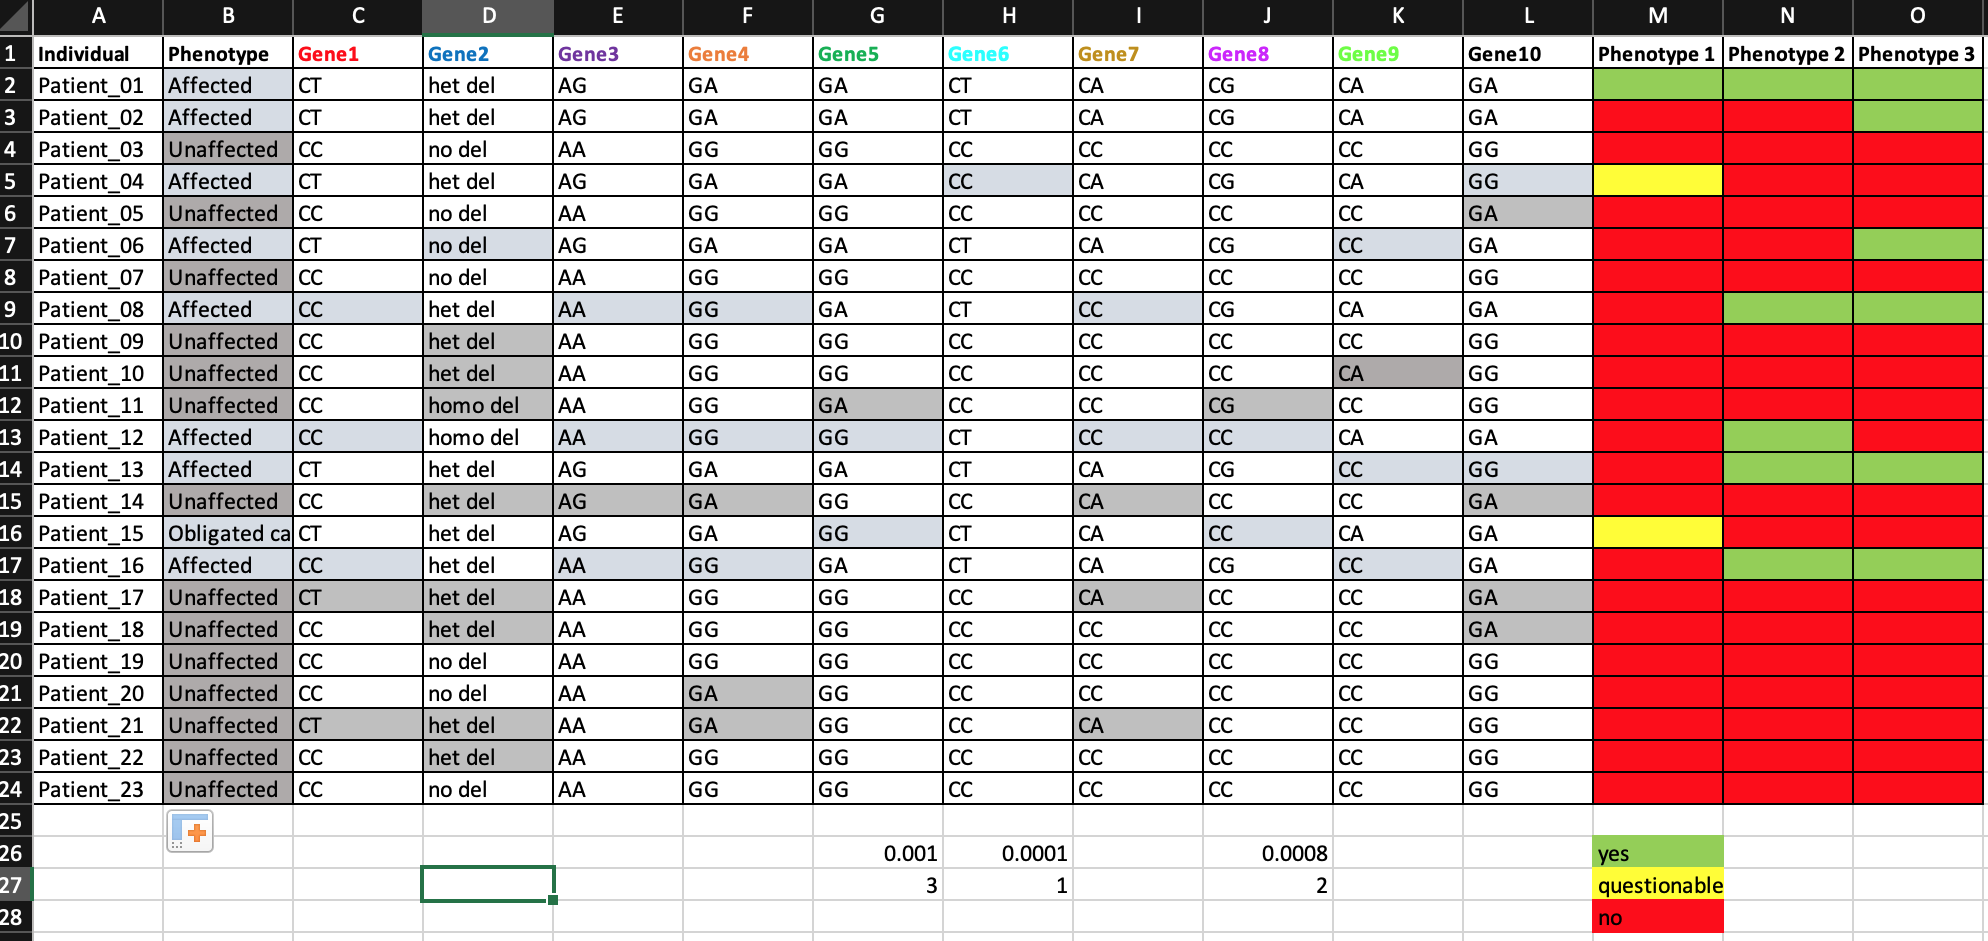
\includegraphics{img/unprocessed_data.png}
\caption{An example adapted from real unprocessed data}
\end{figure}

Instead of Google searching how to handle each step of processing data like this, this chapter will offer a step-by-step outline of the whole game. I will show you what packages and strategies I used to prepare these data for analysis in R.

\hypertarget{start-with-a-sketch}{%
\section{Start with a sketch}\label{start-with-a-sketch}}

When I need to process raw data, I like to begin by sketching the data frame I want to build. Here is a sketch of what I need this data set to look like for analysis:

(As of 2023/06/19, I still need to add this sketch)

\hypertarget{libraries}{%
\section{Libraries}\label{libraries}}

After a sketch, I start with choosing some tools for working with color-coded Excel data. Beside each library I load, I'll comment the reason I find it useful:

\begin{Shaded}
\begin{Highlighting}[]
\CommentTok{\# for data processing }
\FunctionTok{library}\NormalTok{(readxl) }\CommentTok{\# read in .xlsx documents }
\FunctionTok{library}\NormalTok{(dplyr) }\CommentTok{\# transform \& clean data (with \textquotesingle{}pivot\_\textquotesingle{} functions)}
\FunctionTok{library}\NormalTok{(tidyr) }\CommentTok{\# transform \& clean data }
\FunctionTok{library}\NormalTok{(tidyxl) }\CommentTok{\# read in .xlsx *formatting*, including color codes}

\CommentTok{\# for visualization }
\FunctionTok{library}\NormalTok{(ggplot2) }\CommentTok{\# drawing plots }
\FunctionTok{library}\NormalTok{(knitr) }\CommentTok{\# creating tables (has \textquotesingle{}kable()\textquotesingle{} function)}
\FunctionTok{library}\NormalTok{(kableExtra) }\CommentTok{\# making tables pretty }
\FunctionTok{library}\NormalTok{(viridis) }\CommentTok{\# choose color palettes}
\end{Highlighting}
\end{Shaded}

\hypertarget{reading-in-the-data}{%
\section{Reading in the data}\label{reading-in-the-data}}

Here, I read in the data multiple ways to obtain different information. The first line creates \texttt{raw}, which reads in the data without any formatting information. This will make the phenotype columns have all \texttt{NA} values. I need the other \texttt{raw\_} objects to get that information into a workable form.

\begin{Shaded}
\begin{Highlighting}[]
\NormalTok{raw }\OtherTok{\textless{}{-}} \FunctionTok{read\_excel}\NormalTok{(}\AttributeTok{path =} \StringTok{"data/unprocessed\_data\_example.xlsx"}\NormalTok{)}
\NormalTok{raw\_cells }\OtherTok{\textless{}{-}} \FunctionTok{xlsx\_cells}\NormalTok{(}\AttributeTok{path =} \StringTok{"data/unprocessed\_data\_example.xlsx"}\NormalTok{) }
\NormalTok{raw\_formats }\OtherTok{\textless{}{-}} \FunctionTok{xlsx\_formats}\NormalTok{(}\AttributeTok{path =} \StringTok{"data/unprocessed\_data\_example.xlsx"}\NormalTok{) }\CommentTok{\# has color codes }
\NormalTok{raw\_id }\OtherTok{\textless{}{-}}\NormalTok{ raw\_cells[raw\_cells}\SpecialCharTok{$}\NormalTok{col }\SpecialCharTok{==} \DecValTok{1}\NormalTok{, }\FunctionTok{c}\NormalTok{(}\StringTok{"address"}\NormalTok{, }\StringTok{"row"}\NormalTok{, }\StringTok{"col"}\NormalTok{, }\StringTok{"character"}\NormalTok{)]}
\end{Highlighting}
\end{Shaded}

\hypertarget{making-data-long-form}{%
\section{Making data `long form'}\label{making-data-long-form}}

My next step is to transform the data from \href{https://www.statology.org/long-vs-wide-data/\#:~:text=A\%20wide\%20format\%20contains\%20values,repeat\%20in\%20the\%20first\%20column}{wide to long}. The purpose of this is to create visuals later downstream.

\begin{Shaded}
\begin{Highlighting}[]
\CommentTok{\# transform to long}
\NormalTok{long1 }\OtherTok{\textless{}{-}}\NormalTok{ raw }\SpecialCharTok{|\textgreater{}} 
  \FunctionTok{pivot\_longer}\NormalTok{(}\AttributeTok{cols =}\NormalTok{ Gene1}\SpecialCharTok{:}\NormalTok{Gene10,}
               \AttributeTok{names\_to =} \StringTok{"gene"}\NormalTok{,}
               \AttributeTok{values\_to =} \StringTok{"alleles"}\NormalTok{)}
\CommentTok{\# split alleles into two columns  }
\NormalTok{long2 }\OtherTok{\textless{}{-}}\NormalTok{ long1 }\SpecialCharTok{|\textgreater{}} 
  \FunctionTok{mutate}\NormalTok{(}\AttributeTok{allele1 =} \FunctionTok{case\_when}\NormalTok{(}
\NormalTok{    gene }\SpecialCharTok{!=} \StringTok{"Gene2"} \SpecialCharTok{\textasciitilde{}} \FunctionTok{substr}\NormalTok{(alleles, }\DecValTok{1}\NormalTok{,}\DecValTok{1}\NormalTok{),}
\NormalTok{    gene }\SpecialCharTok{==} \StringTok{"Gene2"} \SpecialCharTok{\textasciitilde{}} \ConstantTok{NA\_character\_}
\NormalTok{  ),}
  \AttributeTok{allele2  =} \FunctionTok{case\_when}\NormalTok{(}
\NormalTok{    gene }\SpecialCharTok{!=} \StringTok{"Gene2"} \SpecialCharTok{\textasciitilde{}} \FunctionTok{substr}\NormalTok{(alleles, }\DecValTok{2}\NormalTok{,}\DecValTok{2}\NormalTok{),}
\NormalTok{    gene }\SpecialCharTok{==} \StringTok{"Gene2"} \SpecialCharTok{\textasciitilde{}} \ConstantTok{NA\_character\_}
\NormalTok{  )) }\SpecialCharTok{|\textgreater{}} 
  \CommentTok{\# fix column names to have uniform case }
  \FunctionTok{rename\_with}\NormalTok{(}\AttributeTok{.fn =}\NormalTok{ tolower) }
\end{Highlighting}
\end{Shaded}

\hypertarget{work-with-color-codes}{%
\section{Work with color codes}\label{work-with-color-codes}}

Next, I need to fill in the phenotype information that is color-coded. The colors will be included in \texttt{raw\_formats} as \href{https://www.makeuseof.com/hex-code-what-is-it/}{HEX codes} (without the leading hashtag).

\begin{Shaded}
\begin{Highlighting}[]
\NormalTok{colors }\OtherTok{\textless{}{-}}\NormalTok{ raw\_formats}\SpecialCharTok{$}\NormalTok{local}\SpecialCharTok{$}\NormalTok{fill}\SpecialCharTok{$}\NormalTok{patternFill}\SpecialCharTok{$}\NormalTok{fgColor}\SpecialCharTok{$}\NormalTok{rgb}
\CommentTok{\# NB: colors are given here in order of appearance on the sheet (reading top to bottom)}
\end{Highlighting}
\end{Shaded}

To help me work with the color codes, I wrote a function called \texttt{cells\_by\_color}. \textbf{As soon as you catch yourself being tempted to copy and paste a chunk of code several times, it is time to write a function!}. This is the \emph{most important message} of the tutorial. Data cleaning is a place where there is no room to be sloppy.

\begin{Shaded}
\begin{Highlighting}[]
\CommentTok{\#\textquotesingle{} a function to return the cells of a given color }
\CommentTok{\#\textquotesingle{} @param formats An object returned from tidyxl::xlsx\_formats}
\CommentTok{\#\textquotesingle{} @param cells An object returned from tidyxl::xlsx\_cells}
\CommentTok{\#\textquotesingle{} @param color The hex color WITHOUT the leading "\#" mark}
\CommentTok{\#\textquotesingle{} @return a tibble with the addresses of the cells in that color }
\CommentTok{\#\textquotesingle{} }
\NormalTok{cells\_by\_color }\OtherTok{\textless{}{-}} \ControlFlowTok{function}\NormalTok{(formats, cells, color)\{}
\NormalTok{  colors }\OtherTok{\textless{}{-}}\NormalTok{ formats}\SpecialCharTok{$}\NormalTok{local}\SpecialCharTok{$}\NormalTok{fill}\SpecialCharTok{$}\NormalTok{patternFill}\SpecialCharTok{$}\NormalTok{fgColor}\SpecialCharTok{$}\NormalTok{rgb}
  
\NormalTok{  cells[cells}\SpecialCharTok{$}\NormalTok{local\_format\_id }\SpecialCharTok{\%in\%} \FunctionTok{which}\NormalTok{(colors }\SpecialCharTok{==}\NormalTok{ color), }
                      \FunctionTok{c}\NormalTok{(}\StringTok{"address"}\NormalTok{, }\StringTok{"row"}\NormalTok{, }\StringTok{"col"}\NormalTok{)]}
  
\NormalTok{\}}
\end{Highlighting}
\end{Shaded}

Now, to see my function in action:

\begin{Shaded}
\begin{Highlighting}[]
\CommentTok{\# NB: column M in raw data = phenotypeotype 1}
\CommentTok{\# column N in raw data = phenotypeotype 2}
\CommentTok{\# column O in raw data = phenotypeotype 3}

\NormalTok{green }\OtherTok{\textless{}{-}} \FunctionTok{cells\_by\_color}\NormalTok{(}\AttributeTok{formats =}\NormalTok{ raw\_formats,}
                        \AttributeTok{cells =}\NormalTok{ raw\_cells,}
                        \AttributeTok{color =} \StringTok{"FF92D050"}\NormalTok{) }\SpecialCharTok{|\textgreater{}} 
  \FunctionTok{mutate}\NormalTok{(}\AttributeTok{phenotype =} \FunctionTok{case\_when}\NormalTok{(}
    \FunctionTok{substr}\NormalTok{(address, }\DecValTok{1}\NormalTok{, }\DecValTok{1}\NormalTok{) }\SpecialCharTok{==} \StringTok{"M"} \SpecialCharTok{\textasciitilde{}} \StringTok{"phenotype1"}\NormalTok{,}
    \FunctionTok{substr}\NormalTok{(address, }\DecValTok{1}\NormalTok{, }\DecValTok{1}\NormalTok{) }\SpecialCharTok{==} \StringTok{"N"} \SpecialCharTok{\textasciitilde{}} \StringTok{"phenotype2"}\NormalTok{,}
    \FunctionTok{substr}\NormalTok{(address, }\DecValTok{1}\NormalTok{, }\DecValTok{1}\NormalTok{) }\SpecialCharTok{==} \StringTok{"O"} \SpecialCharTok{\textasciitilde{}} \StringTok{"phenotype3"}
\NormalTok{  ),}
  \AttributeTok{color =} \StringTok{"green"}\NormalTok{)}

\NormalTok{red }\OtherTok{\textless{}{-}} \FunctionTok{cells\_by\_color}\NormalTok{(}\AttributeTok{formats =}\NormalTok{ raw\_formats,}
                      \AttributeTok{cells =}\NormalTok{ raw\_cells,}
                      \AttributeTok{color =} \StringTok{"FFFF0000"}\NormalTok{) }\SpecialCharTok{|\textgreater{}}
  \FunctionTok{mutate}\NormalTok{(}\AttributeTok{phenotype =} \FunctionTok{case\_when}\NormalTok{(}
    \FunctionTok{substr}\NormalTok{(address, }\DecValTok{1}\NormalTok{, }\DecValTok{1}\NormalTok{) }\SpecialCharTok{==} \StringTok{"M"} \SpecialCharTok{\textasciitilde{}} \StringTok{"phenotype1"}\NormalTok{,}
    \FunctionTok{substr}\NormalTok{(address, }\DecValTok{1}\NormalTok{, }\DecValTok{1}\NormalTok{) }\SpecialCharTok{==} \StringTok{"N"} \SpecialCharTok{\textasciitilde{}} \StringTok{"phenotype2"}\NormalTok{,}
    \FunctionTok{substr}\NormalTok{(address, }\DecValTok{1}\NormalTok{, }\DecValTok{1}\NormalTok{) }\SpecialCharTok{==} \StringTok{"O"} \SpecialCharTok{\textasciitilde{}} \StringTok{"phenotype3"}
\NormalTok{  ),}
  \AttributeTok{color =} \StringTok{"red"}\NormalTok{)}


\NormalTok{yellow }\OtherTok{\textless{}{-}} \FunctionTok{cells\_by\_color}\NormalTok{(}\AttributeTok{formats =}\NormalTok{ raw\_formats,}
                         \AttributeTok{cells =}\NormalTok{ raw\_cells,}
                         \AttributeTok{color =} \StringTok{"FFFFFF00"}\NormalTok{) }\SpecialCharTok{|\textgreater{}} 
  \FunctionTok{mutate}\NormalTok{(}\AttributeTok{phenotype =} \FunctionTok{case\_when}\NormalTok{(}
    \FunctionTok{substr}\NormalTok{(address, }\DecValTok{1}\NormalTok{, }\DecValTok{1}\NormalTok{) }\SpecialCharTok{==} \StringTok{"M"} \SpecialCharTok{\textasciitilde{}} \StringTok{"phenotype1"}\NormalTok{,}
    \FunctionTok{substr}\NormalTok{(address, }\DecValTok{1}\NormalTok{, }\DecValTok{1}\NormalTok{) }\SpecialCharTok{==} \StringTok{"N"} \SpecialCharTok{\textasciitilde{}} \StringTok{"phenotype2"}\NormalTok{,}
    \FunctionTok{substr}\NormalTok{(address, }\DecValTok{1}\NormalTok{, }\DecValTok{1}\NormalTok{) }\SpecialCharTok{==} \StringTok{"O"} \SpecialCharTok{\textasciitilde{}} \StringTok{"phenotype3"}
\NormalTok{  ),}
  \AttributeTok{color =} \StringTok{"yellow"}\NormalTok{)}
\end{Highlighting}
\end{Shaded}

With the color codes labeled, I am ready to create a data frame with both genotype and phenotype information:

(As of 2023/06/19, this chapter is still in progress\ldots{} will add more below).

\hypertarget{final-steps}{%
\section{Final steps}\label{final-steps}}

I will write one more function to help me with the last step:

Finally, I have:

\hypertarget{power-and-sample-size-calculations}{%
\chapter{Power and sample size calculations}\label{power-and-sample-size-calculations}}

Power and sample size calculations are a common request for a GRA. In order to estimate the power or calculate the necessary sample size, you will need some measure of \href{https://en.wikipedia.org/wiki/Effect_size}{effect size}. Often, the PI may not have an effect size in mind -- in this case, offer some example scenarios and gauge the PI's reaction. Examples:

\begin{itemize}
\tightlist
\item
  ``If you saw that a subject being treated in group B had a 2 mm increase in the outcome, would you be impressed? Would that be a `big' or notable change?''
\item
  ``How much of an impact would you need to see in order to catch you attention in an abstract? A 50\% increase? Double the outcome?''
\end{itemize}

Your calculations for power/sample size could be done several ways in \texttt{R}: the \texttt{pwr} and \texttt{pwr2} packages can be a good place to start. Suppose you are planning an ANOVA study with these specifications:

\begin{itemize}
\tightlist
\item
  desired power - 85\%
\item
  outcome - 4 level ordered factor which I will treat as numeric (0 - 3)
\item
  main predictor - 3 level factor (treatment A, treatment B, positive control (C))
\item
  desired alpha = 0.05
\end{itemize}

Suppose your PIs don't know what effect size they are looking for, but they do offer some preliminary data from a similar study. Begin with that preliminary data:

\begin{Shaded}
\begin{Highlighting}[]
\FunctionTok{library}\NormalTok{(dplyr)}
\NormalTok{prelim }\OtherTok{\textless{}{-}} \FunctionTok{matrix}\NormalTok{(}\AttributeTok{data =} \FunctionTok{c}\NormalTok{(}\StringTok{"A"}\NormalTok{, }\FloatTok{1.94}\NormalTok{, }\FloatTok{1.20}\NormalTok{,}
                             \StringTok{"A"}\NormalTok{, }\FloatTok{2.75}\NormalTok{, }\FloatTok{0.39}\NormalTok{,}
                             \StringTok{"B"}\NormalTok{, }\FloatTok{0.15}\NormalTok{, }\FloatTok{0.55}\NormalTok{,}
                             \StringTok{"B"}\NormalTok{, }\FloatTok{0.33}\NormalTok{, }\FloatTok{0.74}\NormalTok{),}
                    \AttributeTok{nrow =} \DecValTok{4}\NormalTok{,}
                    \AttributeTok{byrow =}\NormalTok{ T)}
\NormalTok{prelim }\OtherTok{\textless{}{-}}\NormalTok{ prelim }\SpecialCharTok{|\textgreater{}} 
  \FunctionTok{as.data.frame}\NormalTok{() }\SpecialCharTok{|\textgreater{}}
  \FunctionTok{mutate}\NormalTok{(}\FunctionTok{across}\NormalTok{(}\AttributeTok{.cols =} \DecValTok{2}\SpecialCharTok{:}\DecValTok{3}\NormalTok{, }\AttributeTok{.fns =}\NormalTok{ as.numeric)) }\SpecialCharTok{|\textgreater{}}
  \CommentTok{\# collapse isthmus and canal measures, since our study is primarily }
  \CommentTok{\# aimed at comparing treatments A and B with standard of care }
  \FunctionTok{group\_by}\NormalTok{(V1) }\SpecialCharTok{|\textgreater{}} 
  \CommentTok{\# average the mean and sd of each A/B group }
  \FunctionTok{summarise}\NormalTok{(}\AttributeTok{mean =} \FunctionTok{mean}\NormalTok{(V2),}
            \AttributeTok{sd =} \FunctionTok{mean}\NormalTok{(V3))}

\FunctionTok{names}\NormalTok{(prelim) }\OtherTok{\textless{}{-}} \FunctionTok{c}\NormalTok{(}\StringTok{"measure"}\NormalTok{, }\StringTok{"mean"}\NormalTok{, }\StringTok{"sd"}\NormalTok{)}
\end{Highlighting}
\end{Shaded}

Next, you can break down the types of variation:

\begin{Shaded}
\begin{Highlighting}[]
\CommentTok{\# estimate the between group variance to be the variance in mean}
\NormalTok{btw\_group\_var }\OtherTok{\textless{}{-}} \FunctionTok{var}\NormalTok{(prelim}\SpecialCharTok{$}\NormalTok{mean)}

\CommentTok{\# estimate the common variance to be the average of the reported variances }
\NormalTok{within\_group\_var }\OtherTok{\textless{}{-}} \FunctionTok{mean}\NormalTok{((prelim}\SpecialCharTok{$}\NormalTok{sd)}\SpecialCharTok{\^{}}\DecValTok{2}\NormalTok{)}
\end{Highlighting}
\end{Shaded}

After taking these steps, I recommend calculating power using multiple tools and comparing the results you see:

\begin{Shaded}
\begin{Highlighting}[]
\CommentTok{\# using \textquotesingle{}stats\textquotesingle{} package {-} this ships with R}
\FunctionTok{power.anova.test}\NormalTok{(}\AttributeTok{groups =} \DecValTok{3}\NormalTok{,}
                 \AttributeTok{n =} \ConstantTok{NULL}\NormalTok{,}
                 \AttributeTok{between.var =}\NormalTok{ btw\_group\_var,}
                 \AttributeTok{within.var =}\NormalTok{ within\_group\_var,}
                 \AttributeTok{sig.level =} \FloatTok{0.05}\NormalTok{,}
                 \AttributeTok{power =} \FloatTok{0.90}\NormalTok{)}
\end{Highlighting}
\end{Shaded}

\begin{verbatim}
## 
##      Balanced one-way analysis of variance power calculation 
## 
##          groups = 3
##               n = 2.799745
##     between.var = 2.215512
##      within.var = 0.524025
##       sig.level = 0.05
##           power = 0.9
## 
## NOTE: n is number in each group
\end{verbatim}

\begin{Shaded}
\begin{Highlighting}[]
\CommentTok{\# using pwr2}
\FunctionTok{library}\NormalTok{(pwr2)}
\CommentTok{\# using \textquotesingle{}pwr2\textquotesingle{} package }
\FunctionTok{ss.1way}\NormalTok{(}\AttributeTok{k =} \DecValTok{3}\NormalTok{,}
        \AttributeTok{alpha =} \FloatTok{0.05}\NormalTok{,}
        \AttributeTok{beta =} \FloatTok{0.1}\NormalTok{,}
        \AttributeTok{delta =} \FunctionTok{abs}\NormalTok{(}\FunctionTok{diff}\NormalTok{(prelim}\SpecialCharTok{$}\NormalTok{mean)),}
        \AttributeTok{sigma =} \FunctionTok{mean}\NormalTok{(prelim}\SpecialCharTok{$}\NormalTok{sd),}
        \AttributeTok{B =} \DecValTok{100}\NormalTok{)}
\end{Highlighting}
\end{Shaded}

\begin{verbatim}
## 
##      Balanced one-way analysis of variance sample size adjustment 
## 
##               k = 3
##       sig.level = 0.05
##           power = 0.9
##               n = 5
## 
## NOTE: n is number in each group, total sample = 15
\end{verbatim}

The first method estimated that 3 observations would be needed in each group, while the second method estimated this value to be 5. In this case, 5 was a feasible number of observations to achieve, so I reported that value to the PIs. This higher value will also help maintain the level of power desired if I have to pivot to a non-parametric test like the \href{https://en.wikipedia.org/wiki/Kruskal\%E2\%80\%93Wallis_one-way_analysis_of_variance}{Kruskal-Wallis}.

\hypertarget{sas}{%
\section{SAS}\label{sas}}

Note that SAS offers the \texttt{PROC\ POWER} procedure for doing power and sample size calculations. I have often used both R and SAS functions for the same calculation and compared the results. Typically, SAS has much more in-depth documentation -- if you are wondering about the theoretical details for a calculation, SAS documentation is a helpful resource.

\hypertarget{survival-time-to-event-analysis}{%
\chapter{Survival (time-to-event) analysis}\label{survival-time-to-event-analysis}}

Survival analysis is one of the problem-solving settings that separates biostatistics from pure statistics. Survival analysis research questions ask, ``How long until (some event) happens?''. This is a messy question, especially in biomedical research contexts where the investigators do not observe what happens to every observational unit (e.g, every patient) in the study. A patient may come to the clinic once, receive treatment, and then never come back to the clinic again. Whatever outcome the investigators wanted to observe remains unknown for that patient -- we would say the outcome for such a patient is \emph{censored}.

The most-used methods in survival analysis are the \emph{log-rank test} and the \emph{Cox proportional hazards model}. The log-rank test is a conceptual analog to a \href{https://en.wikipedia.org/wiki/Cochran\%E2\%80\%93Mantel\%E2\%80\%93Haenszel_statistics}{Cochran-Mantel-Haenzel test} in categorical data analysis. When working with a survival outcome and a single categorical predictor, the log-rank test can be used to test the null hypothesis: ``there is no difference in survival between the groups being compared.'' The Cox proportional hazards model is a multivariate regression approach in which the exponentiated coefficients are the \emph{hazard ratios}.

{[}ADD A WORD BANK HERE{]}

\hypertarget{assumptionsdiagnostics}{%
\section{Assumptions/diagnostics}\label{assumptionsdiagnostics}}

{[}ADD INFO HERE{]}

\hypertarget{examples}{%
\section{Examples:}\label{examples}}

\begin{itemize}
\item
  Clinical trials: patients battling a chronic condition are randomized to either new drug B or the standard of care drug A. Patients have follow-up visits once per month for 1 year to monitor the time until their symptoms flare up again (e.g., time to relapse or time to recurrence).
\item
  Dentistry: electronic dental records are used to assess the time until re-intervention for crown margin repairs (CMRs). CMRs are compared to assess which materials last longer: glass ionomer, resin-modified glass ionomer, resin-based composite, and amalgam.
\item
  Industry/manufacturing: Suppose there are four machines on a factor floor, two from brand A and two from brand B. The time until next malfunction could be used to compare the two brands of machines.
\end{itemize}

\hypertarget{r-code-tips}{%
\section{R code tips}\label{r-code-tips}}

Packages to know about:

\begin{itemize}
\tightlist
\item
  \texttt{survival}: a must-have for survival analysis
\item
  \texttt{ggsurvfit}: more options for for graphics
\end{itemize}

\hypertarget{references}{%
\section{References}\label{references}}

\begin{itemize}
\item
  Emily Zaboor's \href{https://www.emilyzabor.com/tutorials/survival_analysis_in_r_tutorial.html}{survival analysis tutorial in R}. Good quick-reference for code and plots.
\item
  Patrick Breheny's \href{https://myweb.uiowa.edu/pbreheny/7210/f19/index.html}{publically available course notes for survival analysis}. Lots of examples here, goes in depth in the theory.
\end{itemize}

\hypertarget{survey-data-analysis}{%
\chapter{Survey data analysis}\label{survey-data-analysis}}

One of my more recent projects has involved working with the \href{https://ppc.uiowa.edu/}{UI Public Policy Center} to study data from the \href{https://www.cdc.gov/prams/index.htm}{Pregnancy Risk Assessment and Monitoring System (PRAMS)}. PRAMS contains survey data from participants across the US and its territories. The data I have are a subset of PRAMS that describes participants from specific years who used Medicaid during their pregnancies.

I will give an overview of the tools and tips I have found helpful as I have worked with survey data

\hypertarget{tools-for-analyzing-survey-data}{%
\section{Tools for analyzing survey data}\label{tools-for-analyzing-survey-data}}

\begin{itemize}
\item
  The \href{https://cran.r-project.org/web/packages/survey/index.html}{survey R package} is the classic tool for this type of analysis.
\item
  The \href{https://cran.r-project.org/web/packages/srvyr/vignettes/srvyr-vs-survey.html}{srvyr R package} offers \texttt{tidyverse} syntax of the \texttt{survey} package functions - this was so helpful for subsetting and transforming the data to fit my research objective.
\item
  The \href{https://cran.r-project.org/web/packages/svydiags/index.html}{svydiags R package} offers several functions for model diagnostics with survey data
\end{itemize}

\hypertarget{tips}{%
\section{Tips}\label{tips}}

\begin{enumerate}
\def\labelenumi{\arabic{enumi}.}
\item
  Whenever you subset the data from a survey, you must always consider the survey weights! In R, create a \texttt{svy.design} object \emph{before} you subset.
\item
  The \texttt{gtsummary} package has functions that are designed to present results from a survey - take advantage of this when making tables
\item
  Acronymn to know: ``FPC'' = \textbf{f}inite \textbf{p}opulation \textbf{c}orrection. This is a common variable included in survey data -- if you have this, you should use it when you create your `design' object in \texttt{R}.
\end{enumerate}

\hypertarget{quick-demo}{%
\section{Quick demo}\label{quick-demo}}

Suppose our research question pertains to the academic performance index (api) of elementary schools. Using the \texttt{apipop} data from the \texttt{survey} package, we will investigate this question.

\begin{Shaded}
\begin{Highlighting}[]
\FunctionTok{library}\NormalTok{(survey)}
\FunctionTok{library}\NormalTok{(srvyr)}

\FunctionTok{data}\NormalTok{(api) }\CommentTok{\# data from survey package}

\CommentTok{\# first, create a \textquotesingle{}design\textquotesingle{} object }
\NormalTok{api\_design }\OtherTok{\textless{}{-}}\NormalTok{ apistrat }\SpecialCharTok{|\textgreater{}} 
  \FunctionTok{as\_survey\_design}\NormalTok{(}\AttributeTok{ids =} \DecValTok{0}\NormalTok{, }\CommentTok{\# if there was a clustering variable, it\textquotesingle{}d go here}
                   \AttributeTok{strata =}\NormalTok{ stype, }\CommentTok{\# stratification variable }
                   \AttributeTok{fpc =}\NormalTok{ fpc, }\CommentTok{\# finite population correction }
                   \AttributeTok{weights =}\NormalTok{ pw }\CommentTok{\# survey weights }
\NormalTok{                   )}
\end{Highlighting}
\end{Shaded}

After creating a `design' object, I can filter down to a subset of interest. Supposing I am interested in schools from LA county, I can examine the api of students in LA county alone:

\begin{Shaded}
\begin{Highlighting}[]
\CommentTok{\# look at LA county only }
\NormalTok{la }\OtherTok{\textless{}{-}}\NormalTok{ api\_design }\SpecialCharTok{|\textgreater{}} 
  \FunctionTok{filter}\NormalTok{(cname }\SpecialCharTok{==} \StringTok{"Los Angeles"}\NormalTok{)}

\CommentTok{\# summary table \& bivariate tests }
\FunctionTok{library}\NormalTok{(gtsummary)}
\NormalTok{interest\_vars }\OtherTok{\textless{}{-}} \FunctionTok{c}\NormalTok{(}\StringTok{"pcttest"}\NormalTok{, }\StringTok{"both"}\NormalTok{, }\StringTok{"meals"}\NormalTok{, }\StringTok{"ell"}\NormalTok{, }\StringTok{"yr.rnd"}\NormalTok{, }\StringTok{"mobility"}\NormalTok{,}
                   \StringTok{"avg.ed"}\NormalTok{, }\StringTok{"full"}\NormalTok{,}\StringTok{"enroll"}\NormalTok{, }\StringTok{"api.stu"}\NormalTok{)}
\FunctionTok{tbl\_svysummary}\NormalTok{(la, }
               \CommentTok{\# include only select variables in the table}
               \AttributeTok{include =} \FunctionTok{all\_of}\NormalTok{(interest\_vars),}
               \AttributeTok{by =} \StringTok{"both"}\NormalTok{, }
               \AttributeTok{type =} \FunctionTok{list}\NormalTok{(}\FunctionTok{all\_dichotomous}\NormalTok{() }\SpecialCharTok{\textasciitilde{}} \StringTok{"categorical"}\NormalTok{)) }\SpecialCharTok{|\textgreater{}} 
  \CommentTok{\# formatting }
  \FunctionTok{bold\_labels}\NormalTok{() }\SpecialCharTok{|\textgreater{}} 
  \CommentTok{\# tests}
  \FunctionTok{add\_p}\NormalTok{(}\AttributeTok{test =} \FunctionTok{list}\NormalTok{(}\FunctionTok{all\_categorical}\NormalTok{() }\SpecialCharTok{\textasciitilde{}} \StringTok{"svy.chisq.test"}\NormalTok{,}
                    \FunctionTok{all\_continuous}\NormalTok{() }\SpecialCharTok{\textasciitilde{}} \StringTok{"svy.t.test"}\NormalTok{))}
\end{Highlighting}
\end{Shaded}

\begin{tabular}{l|c|c|c}
\hline
**Characteristic** & **No**, N = 620 & **Yes**, N = 753 & **p-value**\\
\hline
\_\_pcttest\_\_ & 99 (97, 99) & 100 (99, 100) & 0.10\\
\hline
\_\_meals\_\_ & 72 (28, 93) & 60 (35, 82) & 0.8\\
\hline
\_\_ell\_\_ & 23 (10, 34) & 20 (7, 46) & 0.6\\
\hline
\_\_yr.rnd\_\_ &  &  & 0.067\\
\hline
No & 585 (94\%) & 576 (77\%) & \\
\hline
Yes & 35 (5.7\%) & 177 (23\%) & \\
\hline
\_\_mobility\_\_ & 16 (12, 19) & 19 (13, 23) & 0.11\\
\hline
\_\_avg.ed\_\_ & 2.52 (2.20, 3.27) & 2.74 (2.26, 3.35) & 0.6\\
\hline
\_\_full\_\_ & 76 (52, 85) & 74 (67, 87) & 0.2\\
\hline
\_\_enroll\_\_ & 446 (413, 936) & 401 (288, 673) & 0.056\\
\hline
\_\_api.stu\_\_ & 401 (325, 628) & 338 (257, 571) & 0.072\\
\hline
\end{tabular}

\begin{Shaded}
\begin{Highlighting}[]
  \CommentTok{\# NB: survey{-}specific tests available; these tests incorporate/adjust for }
  \CommentTok{\#   survey weights }
\end{Highlighting}
\end{Shaded}

I can also summarize a multivariate model:

\begin{Shaded}
\begin{Highlighting}[]
\NormalTok{lhs }\OtherTok{\textless{}{-}} \FunctionTok{paste}\NormalTok{(interest\_vars, }\AttributeTok{collapse=}\StringTok{"+"}\NormalTok{) }\CommentTok{\# lhs = left hand side (of equation)}
\NormalTok{rhs }\OtherTok{\textless{}{-}} \FunctionTok{paste0}\NormalTok{(}\StringTok{"api99\textasciitilde{}"}\NormalTok{, lhs)}

\NormalTok{fit }\OtherTok{\textless{}{-}} \FunctionTok{lm}\NormalTok{(}\FunctionTok{as.formula}\NormalTok{(rhs),}
          \AttributeTok{data =}\NormalTok{ apistrat)}

\FunctionTok{tbl\_regression}\NormalTok{(fit) }\SpecialCharTok{|\textgreater{}} \FunctionTok{bold\_labels}\NormalTok{()}
\end{Highlighting}
\end{Shaded}

\begin{tabular}{l|c|c|c}
\hline
**Characteristic** & **Beta** & **95\% CI** & **p-value**\\
\hline
\_\_pcttest\_\_ & 1.0 & -1.3, 3.3 & 0.4\\
\hline
\_\_both\_\_ &  &  & \\
\hline
No & — & — & \\
\hline
Yes & -3.2 & -21, 15 & 0.7\\
\hline
\_\_meals\_\_ & -1.6 & -2.2, -0.98 & <0.001\\
\hline
\_\_ell\_\_ & 0.13 & -0.51, 0.77 & 0.7\\
\hline
\_\_yr.rnd\_\_ &  &  & \\
\hline
No & — & — & \\
\hline
Yes & 2.6 & -27, 32 & 0.9\\
\hline
\_\_mobility\_\_ & -0.05 & -0.76, 0.66 & 0.9\\
\hline
\_\_avg.ed\_\_ & 87 & 65, 109 & <0.001\\
\hline
\_\_full\_\_ & 1.5 & 0.81, 2.2 & <0.001\\
\hline
\_\_enroll\_\_ & -0.07 & -0.13, 0.00 & 0.042\\
\hline
\_\_api.stu\_\_ & 0.04 & -0.03, 0.11 & 0.3\\
\hline
\end{tabular}

\hypertarget{longitudinal-data-analysis}{%
\chapter{Longitudinal data analysis}\label{longitudinal-data-analysis}}

\hypertarget{tools-for-longitudinal-data-analysis}{%
\section{Tools for longitudinal data analysis}\label{tools-for-longitudinal-data-analysis}}

\begin{itemize}
\item
  \href{https://cran.r-project.org/web/packages/lme4/index.html}{lme4} R package - fits all your basic linear mixed models
\item
  \href{https://cran.r-project.org/web/packages/nlme/index.html}{nlme} R package - offers functionality for nonlinear mixed effect models
\end{itemize}

\hypertarget{microbiome-data-analysis}{%
\chapter{Microbiome data analysis}\label{microbiome-data-analysis}}

Microbiome data analysis requires working with two separate subtypes of data: the taxonomic data and the sample (meta)data. Taxonomic data is \emph{hierarchical}, meaning that the data are structured in tiers. These tiers are typically the \href{https://en.wikipedia.org/wiki/Operational_taxonomic_unit}{Operational Taxonomic Units} (OTUs). The sample data is the data describing the observations (people or subjects) in the data, and often includes demographic/clinical features.

\hypertarget{tools-for-working-with-microbiome-data}{%
\section{Tools for working with microbiome data}\label{tools-for-working-with-microbiome-data}}

\begin{itemize}
\tightlist
\item
  \href{https://grunwaldlab.github.io/metacoder_documentation/}{metacoder} and \href{https://docs.ropensci.org/taxa/}{taxa} are \texttt{R} packages built on previous packages \href{https://peat-clark.github.io/BIO381/veganTutorial.html}{vegan} and \href{https://vaulot.github.io/tutorials/Phyloseq_tutorial.html\#phyloseq-r-library}{phyloseq}. All of these links include tutorials for working with taxonomic data.
\end{itemize}

\hypertarget{genetics-gwas-data-analysis}{%
\chapter{Genetics (GWAS) data analysis}\label{genetics-gwas-data-analysis}}

The rate at which new tools for GWAS data analysis are created is mind-boggling. It seems like a new paper in this area comes out each week -- which makes it a challenge to summarize the tools available for working in this area. With this in mind, consider the set of tools and tips provided here as select suggestions from my own experience rather than an exhaustive list.

\hypertarget{r-packages}{%
\section{R packages}\label{r-packages}}

\begin{itemize}
\item
  \href{https://privefl.github.io/bigsnpr/index.html}{bigsnpr} - a relatively new package that offers functions for manipulating PLINK data files, doing \protect\hyperlink{acronyms}{QC} and relatedness/imputation, pruning/clumping and correlation analysis, and calculation of polygenic scores. Functions for basic marginal association analysis are also available.
\item
  \href{https://www.bioconductor.org/packages/release/bioc/html/snpStats.html}{snpStats} - an older, widely-used Bioconductor package that has functions for doing QC, imputation, and marginal association analysis. Note: this package is not as memory efficient as \texttt{bigsnpr}.
\item
  \href{https://pbreheny.github.io/ncvreg/}{ncvreg} - a newer package that implements penalized regression models for high dimensional data. TL;DR: this package will allow you to analyze SNPs (or whatever the features of the data are) \emph{jointly}, taking into account the relationships between them. This is in stark contrast to the marginal (one-feature-at-a-time) approaches that are widely used. A note for the stats nerds: unlike the popular \href{https://glmnet.stanford.edu/articles/glmnet.html\#:~:text=Glmnet\%20is\%20a\%20package\%20that,for\%20the\%20regularization\%20parameter\%20lambda.}{glmnet} package, \texttt{ncvreg} offers non-convex penalties in addition to the lasso.
\item
  \href{https://areisett.github.io/penalizedLMM/}{penalizedLMM} - an in-development package for joint analysis of features in contexts where the data are structured (e.g., admixed populations, family-based GWAS data, etc.). This package has contributions from several of \href{https://myweb.uiowa.edu/pbreheny/students.html}{Patrick Breheny's doc students} (including me).
\item
  \href{https://cran.r-project.org/web/packages/qqman/}{qqman} - a package for creating QQ plots and Manhattan plots from GWAS analysis results.
\item
  \href{https://github.com/YinLiLin/CMplot}{CMplot} - a package for creating `fancy' QQ plots and Manhattan plots, including those that are circular. This package offers many customization options for annotation these plots.
\item
  \href{https://github.com/RayDebashree/PLACO}{PLACO}: this isn't a `package' \emph{per se}, but this method for assessing pleiotropy between traits is implemented in \texttt{R}.
\end{itemize}

\hypertarget{command-line-tools}{%
\section{Command-line tools}\label{command-line-tools}}

\begin{itemize}
\item
  \href{https://www.cog-genomics.org/plink/1.9/}{PLINK}
\item
  \href{https://github.com/bulik/ldsc/wiki/Heritability-and-Genetic-Correlation}{LDSC}
\end{itemize}

\hypertarget{geographic-gis-data-analysis}{%
\chapter{Geographic (GIS) data analysis}\label{geographic-gis-data-analysis}}

In a couple of my projects, I have had the opportunity to visualize data using maps at the county level. Here is an example of the sort of maps I have made, using some simulated data.

Suppose that a PI wants to study access to care through teledentistry. The specific research question is something like, ``in a population of patients treated at my dental clinic from January 2021 - May 2023, what were the patterns in the relationships between 1) the distance traveled to the clinic, 2) the mode of the intake exam (in-person or virtual), and 3) treatment completion within 6 months (yes or no). Suppose further that I (the analyst) have access to the county in which each person lives, in addition to the clinical information relevant to our research in the electronic dental records.

The first thing I would do is look online to find \href{https://geodata.iowa.gov/datasets/iowa::iowa-county-boundaries/explore?location=42.011193\%2C-93.543500\%2C8.00}{publicly available data} with \href{https://en.wikipedia.org/wiki/FIPS_county_code}{Federal Information Processing Standard (FIPS) codes} for Iowa at the county level. I will use the R package \texttt{sf} to handle GIS data, which often comes in \texttt{.shp} or \texttt{GeoJSON} formats. Data in these sorts of files have what we need to draw a map of Iowa with the counties demarcated on the map.

\begin{Shaded}
\begin{Highlighting}[]
\FunctionTok{library}\NormalTok{(sf) }\CommentTok{\# package for GIS data }
\end{Highlighting}
\end{Shaded}

\begin{verbatim}
## Linking to GEOS 3.10.2, GDAL 3.4.2, PROJ 8.2.1; sf_use_s2() is TRUE
\end{verbatim}

\begin{Shaded}
\begin{Highlighting}[]
\NormalTok{ia }\OtherTok{\textless{}{-}} \FunctionTok{st\_read}\NormalTok{(}\StringTok{"data/Iowa\_County\_Boundaries.geojson"}\NormalTok{)}
\end{Highlighting}
\end{Shaded}

\begin{verbatim}
## Reading layer `IowaCounties' from data source 
##   `/Users/tabithapeter/Desktop/train_gra/data/Iowa_County_Boundaries.geojson' 
##   using driver `GeoJSON'
## Simple feature collection with 99 features and 9 fields
## Geometry type: MULTIPOLYGON
## Dimension:     XY
## Bounding box:  xmin: -96.63944 ymin: 40.37566 xmax: -90.1401 ymax: 43.50109
## Geodetic CRS:  WGS 84
\end{verbatim}

\begin{Shaded}
\begin{Highlighting}[]
\NormalTok{ia\_geom }\OtherTok{\textless{}{-}} \FunctionTok{st\_geometry}\NormalTok{(ia)}


\CommentTok{\# check {-} a test plot to make sure the map looks right. }
\FunctionTok{par}\NormalTok{(}\AttributeTok{mar =} \FunctionTok{c}\NormalTok{(}\DecValTok{0}\NormalTok{,}\DecValTok{0}\NormalTok{,}\DecValTok{1}\NormalTok{,}\DecValTok{0}\NormalTok{))}
\FunctionTok{plot}\NormalTok{(ia[}\DecValTok{1}\NormalTok{], }\AttributeTok{reset =} \ConstantTok{FALSE}\NormalTok{) }\CommentTok{\# reset = FALSE: we want to add to a plot with a legend}
\FunctionTok{plot}\NormalTok{(ia[}\DecValTok{1}\NormalTok{,}\DecValTok{1}\NormalTok{], }\AttributeTok{col =} \StringTok{\textquotesingle{}grey\textquotesingle{}}\NormalTok{, }\AttributeTok{add =} \ConstantTok{TRUE}\NormalTok{)}
\end{Highlighting}
\end{Shaded}

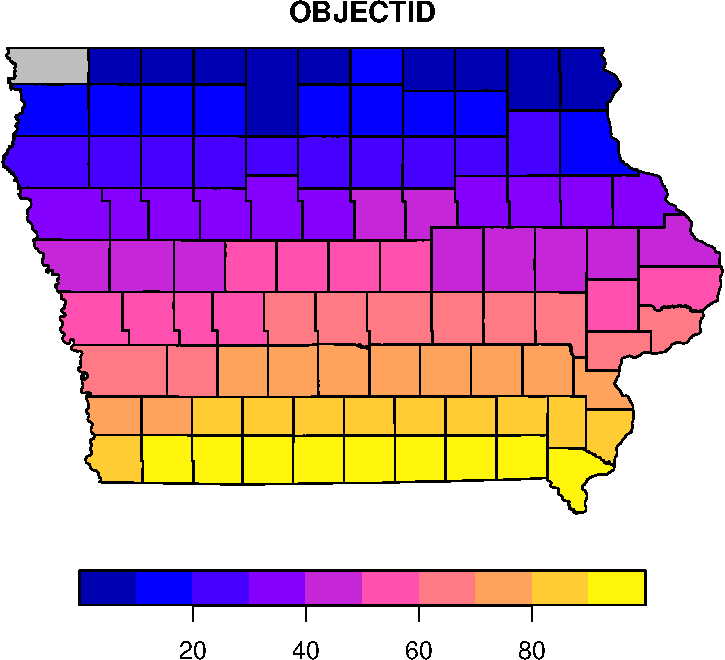
\includegraphics{_main_files/figure-latex/unnamed-chunk-24-1.pdf}
This sample map is the correct shape -- here, the 99 counties are colored according to their index (1-99). We want to make a map where the colors correspond to the number of patients representing each county.

Supposing one has access to electronic dental records, the data for such a study may look like this:

\begin{Shaded}
\begin{Highlighting}[]
\CommentTok{\# simulate data}
\FunctionTok{library}\NormalTok{(dplyr)}
\NormalTok{key }\OtherTok{\textless{}{-}} \FunctionTok{read.csv}\NormalTok{(}\StringTok{"data/ia\_counties.csv"}\NormalTok{) }\SpecialCharTok{|\textgreater{}} 
  \CommentTok{\# narrow down to only IA (for sake of example)}
  \FunctionTok{filter}\NormalTok{(State }\SpecialCharTok{==} \StringTok{"IA"}\NormalTok{) }\CommentTok{\# gives me county names }



\CommentTok{\# TD = teledentistry}
\FunctionTok{set.seed}\NormalTok{(}\DecValTok{52242}\NormalTok{) }
\NormalTok{td }\OtherTok{\textless{}{-}} \FunctionTok{data.frame}\NormalTok{(}
  \AttributeTok{id =} \DecValTok{1}\SpecialCharTok{:}\DecValTok{1000}\NormalTok{,}
  \AttributeTok{year =} \FunctionTok{sample}\NormalTok{(}\DecValTok{2021}\SpecialCharTok{:}\DecValTok{2023}\NormalTok{, }\DecValTok{1000}\NormalTok{, }\AttributeTok{replace =} \ConstantTok{TRUE}\NormalTok{),}
  \AttributeTok{complete =} \FunctionTok{sample}\NormalTok{(}\DecValTok{0}\SpecialCharTok{:}\DecValTok{1}\NormalTok{, }\DecValTok{1000}\NormalTok{, }\AttributeTok{replace =} \ConstantTok{TRUE}\NormalTok{),}
  \AttributeTok{county =} \FunctionTok{sample}\NormalTok{(key}\SpecialCharTok{$}\NormalTok{NAME, }\DecValTok{1000}\NormalTok{, }\AttributeTok{replace =} \ConstantTok{TRUE}\NormalTok{),}
  \AttributeTok{mode =} \FunctionTok{sample}\NormalTok{(}\FunctionTok{c}\NormalTok{(}\StringTok{"virtual"}\NormalTok{, }\StringTok{"in{-}person"}\NormalTok{), }\DecValTok{1000}\NormalTok{, }\AttributeTok{replace =} \ConstantTok{TRUE}\NormalTok{)}
\NormalTok{)}

\FunctionTok{library}\NormalTok{(knitr)}
\FunctionTok{head}\NormalTok{(td) }\SpecialCharTok{|\textgreater{}}
  \FunctionTok{kable}\NormalTok{(}\AttributeTok{caption =} \StringTok{"Simulated data from electronic dental records"}\NormalTok{)}
\end{Highlighting}
\end{Shaded}

\begin{table}

\caption{\label{tab:unnamed-chunk-25}Simulated data from electronic dental records}
\centering
\begin{tabular}[t]{r|r|r|l|l}
\hline
id & year & complete & county & mode\\
\hline
1 & 2021 & 0 & Howard & virtual\\
\hline
2 & 2021 & 1 & Clay & in-person\\
\hline
3 & 2021 & 0 & Palo Alto & virtual\\
\hline
4 & 2022 & 0 & Buchanan & virtual\\
\hline
5 & 2022 & 0 & O'Brien & virtual\\
\hline
6 & 2023 & 1 & Floyd & virtual\\
\hline
\end{tabular}
\end{table}

Now, I am ready to create a map that will communicate to my collaborators where our patients are driving from to receive their treatment.

\begin{Shaded}
\begin{Highlighting}[]
\CommentTok{\# determine how many patients in each county}
\NormalTok{td\_summarize }\OtherTok{\textless{}{-}}\NormalTok{ td }\SpecialCharTok{|\textgreater{}}
    \FunctionTok{group\_by}\NormalTok{(county) }\SpecialCharTok{|\textgreater{}}
    \FunctionTok{summarise}\NormalTok{(}\AttributeTok{N =} \FunctionTok{n}\NormalTok{()) }\SpecialCharTok{\%\textgreater{}\%}
  \FunctionTok{ungroup}\NormalTok{()}

\CommentTok{\# add fips codes (from GeoJSON file)}
\NormalTok{td\_summarize }\OtherTok{\textless{}{-}} \FunctionTok{right\_join}\NormalTok{(td\_summarize, ia,}
            \AttributeTok{by =} \FunctionTok{c}\NormalTok{(}\StringTok{"county"} \OtherTok{=} \StringTok{"CountyName"}\NormalTok{)) }

\CommentTok{\# create sf object (for drawing a map)}
\NormalTok{map }\OtherTok{\textless{}{-}}\NormalTok{ td\_summarize }\SpecialCharTok{\%\textgreater{}\%}
  \FunctionTok{st\_as\_sf}\NormalTok{()}

\CommentTok{\# draw the map }
\FunctionTok{library}\NormalTok{(ggplot2)}
\FunctionTok{library}\NormalTok{(viridis)}
\FunctionTok{ggplot}\NormalTok{() }\SpecialCharTok{+} 
  \FunctionTok{geom\_sf}\NormalTok{(}\AttributeTok{data =}\NormalTok{ map,}
          \FunctionTok{aes}\NormalTok{(}\AttributeTok{fill =}\NormalTok{ N)) }\SpecialCharTok{+} 
  \FunctionTok{scale\_fill\_viridis}\NormalTok{() }\SpecialCharTok{+} 
  \FunctionTok{labs}\NormalTok{(}\AttributeTok{title =} \StringTok{"Map of IA Residents by County"}\NormalTok{, }\AttributeTok{fill =} \StringTok{"Number of }\SpecialCharTok{\textbackslash{}n}\StringTok{patients"}\NormalTok{) }\SpecialCharTok{+}
  \FunctionTok{theme\_bw}\NormalTok{() }
\end{Highlighting}
\end{Shaded}

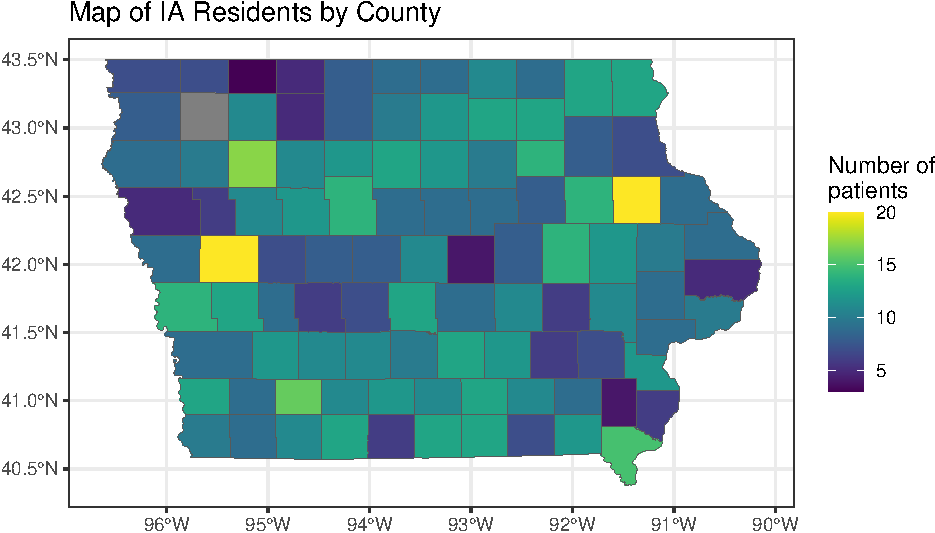
\includegraphics{_main_files/figure-latex/unnamed-chunk-26-1.pdf}

  \bibliography{book.bib}

\end{document}
